\section{Results}
In this section the results of the thesis work is presented. First we will take a look at some examples images from two endoscopy videos to familiarize ourselves a little with the data the models have been trained on. We will then look at the model selection and how the best performing model was chosen, followed by the separation point predictions of the post-processing approaches. Next we look at the treatment predictions from the segmentation results of the 2D ResNet, before we try and refine these results by a using U-Net model. To end with, we use the U-Net segmentations for treatment predictions. 

In \autoref{exampleFrames} we see four examples of training data from two different endoscopy videos and two different patients. In the left column we have examples of inflamed bowel tissue and in the right column examples of healthy bowel tissue. The top row of images is from the same video and likewise, the bottom row of images is from the same video. We note how even though the image pairs comes from the same patient, the colouring of the bowel tissue can change quite a lot throughout a video, which especially is seen in the bottom row of images. We also note, how much the colon twists has a large impact on the lighting, and thus on the colouring of the tissue. And lastly we also see from image (a) and (d) how similar healthy and inflamed tissue can look. 

\begin{figure}[H]
	\centering
	\begin{subfigure}{0.4\linewidth}
		\centering
		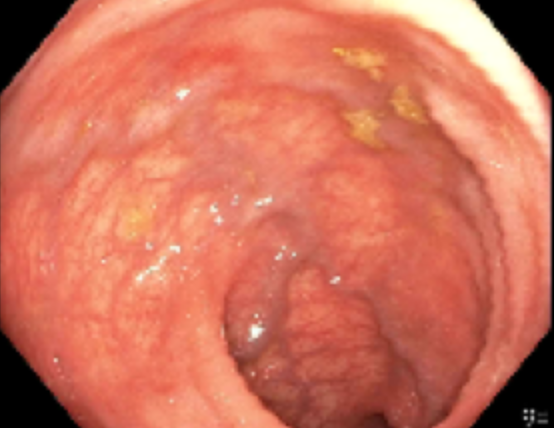
\includegraphics[width=\linewidth]{Materials/Results/Intro/idx_1_frame_830}
		\caption{Inflamed example image from validation video.}
	\end{subfigure}
	\hspace{0.5cm}
	\begin{subfigure}{0.4\linewidth}
		\centering
		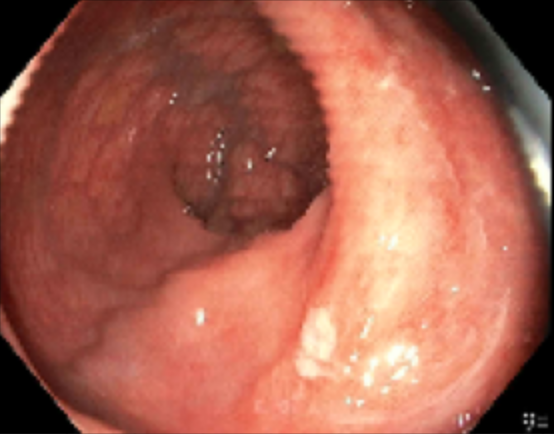
\includegraphics[width=\linewidth]{Materials/Results/Intro/idx_1_frame_1210}
		\caption{Healthy example image from validation video.\newline}
	\end{subfigure}
	\\
	\begin{subfigure}{0.4\linewidth}
		\centering
		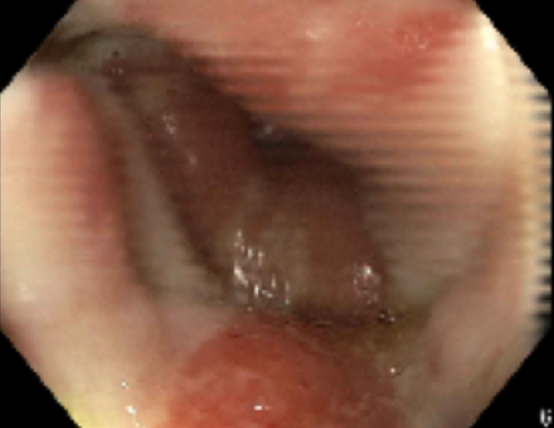
\includegraphics[width=\linewidth]{Materials/Results/Intro/idx_4_frame_800}
		\caption{Inflamed example image.}
	\end{subfigure}
	\hspace{0.5cm}
	\begin{subfigure}{0.4\linewidth}
		\centering
		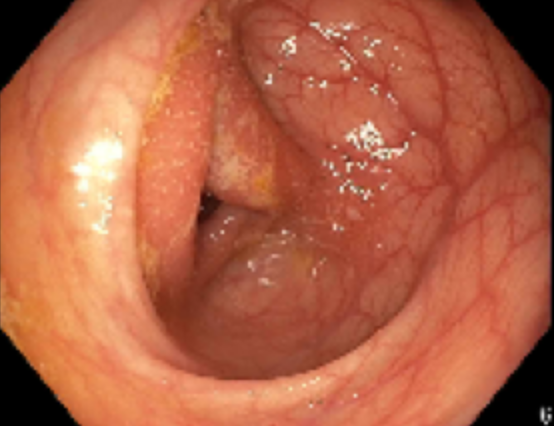
\includegraphics[width=\linewidth]{Materials/Results/Intro/idx_4_frame_3000}
		\caption{Healthy example image.}
	\end{subfigure}
	\caption{Examples images from two endoscopy videos.}
	\label{exampleFrames}
\end{figure}

\subsection{Model evaluation and selection} \label{modelRes}
Training was conducted by training several 2D ResNet models, one for each of the datasets, and using a single video as a constant validation set to tune learning rate, weight decay and the dropout layers. For loss functions binary cross entropy was used and for optimization Adam was used. Each model was trained for 65 epochs with a learning rate of $10^{-5}$. No weight decay was added. The true segmentations was 'artificially' constructed by concatenating a vector of zeros equal in length to the number of frames up to the true separation point, and a vector of ones equal in length to the remaining frames of the video, such that we get one continuous block of inflammation predictions followed by one continuous block of healthy predictions which correspond to how the doctor annotated the video.\\ 
In this section two results will be reported. First a five fold approach used to evaluate the model performance where each dataset is split in five folds, then a model is trained on four folds and evaluated on the constant validation set. Second, models are trained on all the data from each dataset respectively, and then used to predict each frame in the validation set for visual inspection.

\begin{table}[H]
	\hspace{-2.2cm}
	\begin{tabular}{|l|cc|cc|cc|cc|cc|r|r|r|}
		\hline
		\multicolumn{1}{|c|}{Dataset}    & \multicolumn{2}{c|}{Fold 1}                                                                                                     & \multicolumn{2}{c|}{Fold 2}                                                                                                     & \multicolumn{2}{c|}{Fold 3}                                                                                                     & \multicolumn{2}{c|}{Fold 4}                                                                                                     & \multicolumn{2}{c|}{Fold 5}                                                                                                     & \multicolumn{1}{c|}{Avg. T}           & \multicolumn{1}{c|}{Avg. V}           & \multicolumn{1}{c|}{Frames} \\ \hline
		\multicolumn{1}{|c|}{}           & \multicolumn{1}{c|}{T}                                                    & V                                                   & \multicolumn{1}{c|}{T}                                                    & V                                                   & \multicolumn{1}{c|}{T}                                                    & V                                                   & \multicolumn{1}{c|}{T}                                                    & V                                                   & \multicolumn{1}{c|}{T}                                                    & V                                                   & \multicolumn{1}{l|}{}                 & \multicolumn{1}{l|}{}                 & \multicolumn{1}{l|}{}       \\ \hline
		Idx\_4\_skip\_10                 & \multicolumn{1}{c|}{\cellcolor[HTML]{FFC7CE}{\color[HTML]{9C0006} 100.0}} & \cellcolor[HTML]{C6EFCE}{\color[HTML]{006100} 67.9} & \multicolumn{1}{c|}{\cellcolor[HTML]{FFC7CE}{\color[HTML]{9C0006} 100.0}} & \cellcolor[HTML]{C6EFCE}{\color[HTML]{006100} 33.2} & \multicolumn{1}{c|}{\cellcolor[HTML]{FFC7CE}{\color[HTML]{9C0006} 100.0}} & \cellcolor[HTML]{C6EFCE}{\color[HTML]{006100} 35.5} & \multicolumn{1}{c|}{\cellcolor[HTML]{FFC7CE}{\color[HTML]{9C0006} 100.0}} & \cellcolor[HTML]{C6EFCE}{\color[HTML]{006100} 43.1} & \multicolumn{1}{c|}{\cellcolor[HTML]{FFC7CE}{\color[HTML]{9C0006} 100.0}} & \cellcolor[HTML]{C6EFCE}{\color[HTML]{006100} 45.9} & {\color[HTML]{7F7F7F} \textit{100}}   & {\color[HTML]{7F7F7F} \textit{45.12}} & 499                         \\ \hline
		Idx\_4\_5\_skip\_20              & \multicolumn{1}{c|}{\cellcolor[HTML]{FFC7CE}{\color[HTML]{9C0006} 99.2}}  & \cellcolor[HTML]{C6EFCE}{\color[HTML]{006100} 47.2} & \multicolumn{1}{c|}{\cellcolor[HTML]{FFC7CE}{\color[HTML]{9C0006} 100.0}} & \cellcolor[HTML]{C6EFCE}{\color[HTML]{006100} 41.0} & \multicolumn{1}{c|}{\cellcolor[HTML]{FFC7CE}{\color[HTML]{9C0006} 99.8}}  & \cellcolor[HTML]{C6EFCE}{\color[HTML]{006100} 35.6} & \multicolumn{1}{c|}{\cellcolor[HTML]{FFC7CE}{\color[HTML]{9C0006} 100.0}} & \cellcolor[HTML]{C6EFCE}{\color[HTML]{006100} 39.0} & \multicolumn{1}{c|}{\cellcolor[HTML]{FFC7CE}{\color[HTML]{9C0006} 99.5}}  & \cellcolor[HTML]{C6EFCE}{\color[HTML]{006100} 33.0} & {\color[HTML]{7F7F7F} \textit{99.7}}  & {\color[HTML]{7F7F7F} \textit{39.16}} & 500                         \\ \hline
		Idx\_2\_3\_4\_5\_6\_skip\_50     & \multicolumn{1}{c|}{\cellcolor[HTML]{FFC7CE}{\color[HTML]{9C0006} 99.5}}  & \cellcolor[HTML]{C6EFCE}{\color[HTML]{006100} 71.4} & \multicolumn{1}{c|}{\cellcolor[HTML]{FFC7CE}{\color[HTML]{9C0006} 99.5}}  & \cellcolor[HTML]{C6EFCE}{\color[HTML]{006100} 63.7} & \multicolumn{1}{c|}{\cellcolor[HTML]{FFC7CE}{\color[HTML]{9C0006} 99.5}}  & \cellcolor[HTML]{C6EFCE}{\color[HTML]{006100} 70.0} & \multicolumn{1}{c|}{\cellcolor[HTML]{FFC7CE}{\color[HTML]{9C0006} 99.7}}  & \cellcolor[HTML]{C6EFCE}{\color[HTML]{006100} 45.5} & \multicolumn{1}{c|}{\cellcolor[HTML]{FFC7CE}{\color[HTML]{9C0006} 100.0}} & \cellcolor[HTML]{C6EFCE}{\color[HTML]{006100} 43.4} & {\color[HTML]{7F7F7F} \textit{99.64}} & {\color[HTML]{7F7F7F} \textit{58.8}}  & 491                         \\ \hline
		Idx\_2\_3\_4\_5\_6\_skip\_20     & \multicolumn{1}{c|}{\cellcolor[HTML]{FFC7CE}{\color[HTML]{9C0006} 100.0}} & \cellcolor[HTML]{C6EFCE}{\color[HTML]{006100} 60.9} & \multicolumn{1}{c|}{\cellcolor[HTML]{FFC7CE}{\color[HTML]{9C0006} 99.7}}  & \cellcolor[HTML]{C6EFCE}{\color[HTML]{006100} 61.8} & \multicolumn{1}{c|}{\cellcolor[HTML]{FFC7CE}{\color[HTML]{9C0006} 99.7}}  & \cellcolor[HTML]{C6EFCE}{\color[HTML]{006100} 66.2} & \multicolumn{1}{c|}{\cellcolor[HTML]{FFC7CE}{\color[HTML]{9C0006} 99.7}}  & \cellcolor[HTML]{C6EFCE}{\color[HTML]{006100} 71.4} & \multicolumn{1}{c|}{\cellcolor[HTML]{FFC7CE}{\color[HTML]{9C0006} 99.8}}  & \cellcolor[HTML]{C6EFCE}{\color[HTML]{006100} 65.5} & {\color[HTML]{7F7F7F} \textit{99.78}} & {\color[HTML]{7F7F7F} \textit{65.16}} & 1226                        \\ \hline
		Idx\_4\_14\_18\_20\_32\_skip\_20 & \multicolumn{1}{c|}{\cellcolor[HTML]{FFC7CE}{\color[HTML]{9C0006} 99.7}}  & \cellcolor[HTML]{C6EFCE}{\color[HTML]{006100} 33.9} & \multicolumn{1}{c|}{\cellcolor[HTML]{FFC7CE}{\color[HTML]{9C0006} 100.0}} & \cellcolor[HTML]{C6EFCE}{\color[HTML]{006100} 42.6} & \multicolumn{1}{c|}{\cellcolor[HTML]{FFC7CE}{\color[HTML]{9C0006} 99.9}}  & \cellcolor[HTML]{C6EFCE}{\color[HTML]{006100} 40.6} & \multicolumn{1}{c|}{\cellcolor[HTML]{FFC7CE}{\color[HTML]{9C0006} 99.9}}  & \cellcolor[HTML]{C6EFCE}{\color[HTML]{006100} 37.2} & \multicolumn{1}{c|}{\cellcolor[HTML]{FFC7CE}{\color[HTML]{9C0006} 99.8}}  & \cellcolor[HTML]{C6EFCE}{\color[HTML]{006100} 38.2} & {\color[HTML]{7F7F7F} \textit{99.86}} & {\color[HTML]{7F7F7F} \textit{38.5}}  & 997                         \\ \hline
		Idx\_4\_14\_18\_20\_32\_skip\_5  & \multicolumn{1}{c|}{\cellcolor[HTML]{FFC7CE}{\color[HTML]{9C0006} 99.9}}  & \cellcolor[HTML]{C6EFCE}{\color[HTML]{006100} 69.3} & \multicolumn{1}{c|}{\cellcolor[HTML]{FFC7CE}{\color[HTML]{9C0006} 100.0}} & \cellcolor[HTML]{C6EFCE}{\color[HTML]{006100} 57.1} & \multicolumn{1}{c|}{\cellcolor[HTML]{FFC7CE}{\color[HTML]{9C0006} 86.4}}  & \cellcolor[HTML]{C6EFCE}{\color[HTML]{006100} 39.5} & \multicolumn{1}{c|}{\cellcolor[HTML]{FFC7CE}{\color[HTML]{9C0006} 99.5}}  & \cellcolor[HTML]{C6EFCE}{\color[HTML]{006100} 55.9} & \multicolumn{1}{c|}{\cellcolor[HTML]{FFC7CE}{\color[HTML]{9C0006} 99.9}}  & \cellcolor[HTML]{C6EFCE}{\color[HTML]{006100} 60.9} & {\color[HTML]{7F7F7F} \textit{97.14}} & {\color[HTML]{7F7F7F} \textit{56.54}} & 3978                        \\ \hline
		Idx\_3\_23\_skip\_10             & \multicolumn{1}{c|}{\cellcolor[HTML]{FFC7CE}{\color[HTML]{9C0006} 100.0}} & \cellcolor[HTML]{C6EFCE}{\color[HTML]{006100} 72.0} & \multicolumn{1}{c|}{\cellcolor[HTML]{FFC7CE}{\color[HTML]{9C0006} 100.0}} & \cellcolor[HTML]{C6EFCE}{\color[HTML]{006100} 72.3} & \multicolumn{1}{c|}{\cellcolor[HTML]{FFC7CE}{\color[HTML]{9C0006} 100.0}} & \cellcolor[HTML]{C6EFCE}{\color[HTML]{006100} 72.6} & \multicolumn{1}{c|}{\cellcolor[HTML]{FFC7CE}{\color[HTML]{9C0006} 100.0}} & \cellcolor[HTML]{C6EFCE}{\color[HTML]{006100} 72.4} & \multicolumn{1}{c|}{\cellcolor[HTML]{FFC7CE}{\color[HTML]{9C0006} 100.0}} & \cellcolor[HTML]{C6EFCE}{\color[HTML]{006100} 70.6} & {\color[HTML]{7F7F7F} \textit{100.0}} & {\color[HTML]{7F7F7F} \textit{72.0}}  & 829                         \\ \hline
		Idx\_19\_24\_skip\_5             & \multicolumn{1}{c|}{\cellcolor[HTML]{FFC7CE}{\color[HTML]{9C0006} 100.0}} & \cellcolor[HTML]{C6EFCE}{\color[HTML]{006100} 26.8} & \multicolumn{1}{c|}{\cellcolor[HTML]{FFC7CE}{\color[HTML]{9C0006} 100.0}} & \cellcolor[HTML]{C6EFCE}{\color[HTML]{006100} 25.9} & \multicolumn{1}{c|}{\cellcolor[HTML]{FFC7CE}{\color[HTML]{9C0006} 99.8}}  & \cellcolor[HTML]{C6EFCE}{\color[HTML]{006100} 27.7} & \multicolumn{1}{c|}{\cellcolor[HTML]{FFC7CE}{\color[HTML]{9C0006} 100.0}} & \cellcolor[HTML]{C6EFCE}{\color[HTML]{006100} 27.3} & \multicolumn{1}{c|}{\cellcolor[HTML]{FFC7CE}{\color[HTML]{9C0006} 100.0}} & \cellcolor[HTML]{C6EFCE}{\color[HTML]{006100} 26.7} & {\color[HTML]{7F7F7F} \textit{100.0}} & {\color[HTML]{7F7F7F} \textit{26.9}}  & 600                         \\ \hline
	\end{tabular}
	\caption{Evaluation results for training a modified 2D ResNet on different datasets. All results are in percent. At each fold, T stands for training accuracy and V stands for validation accuracy.}
	\label{2dresnetevalres}
\end{table}

In \autoref{2dresnetevalres} we see the evaluation of the five fold approach. T stands for training accuracy and V stands for validation accuracy. All results are reported in percent. We note dataset \textit{Idx\_3\_23\_skip\_10} and \textit{Idx\_2\_3\_4\_5\_6\_skip\_20} have the highest validation accuracies while \textit{Idx\_19\_24\_skip\_5} has the lowest followed by \textit{Idx\_4\_14\_18\_20\_32\_} \textit{skip\_5}. We also note there seemingly is no relation between the sheer number of training images and high validation accuracy, but there is some relation when we chose to add more images from the same dataset. Likewise there is seemingly no relation between the different number of patients the training images comes from and high validation accuracy.

To assert whether the reported accuracies are accurate, we will now take a look at how the models predicted on some videos. First we will look at how each of the models predicted on the validation video to establish a baseline. The results can be seen in \autoref{firstfive} and in \autoref{lastthree}. For each illustration the true segmentation of the video has been drawn as the first bar. For these results, this means approximately 72\% of the frames are annotated as inflamed and the last frames as healthy. The second bar is the model predictions. The blue line indicates the models' confidence in a healthy prediction, and a probability above 50\% means it has predicted the frame is healthy.

\begin{figure}[H]
	\centering
	\begin{subfigure}{\linewidth}
		\centering
		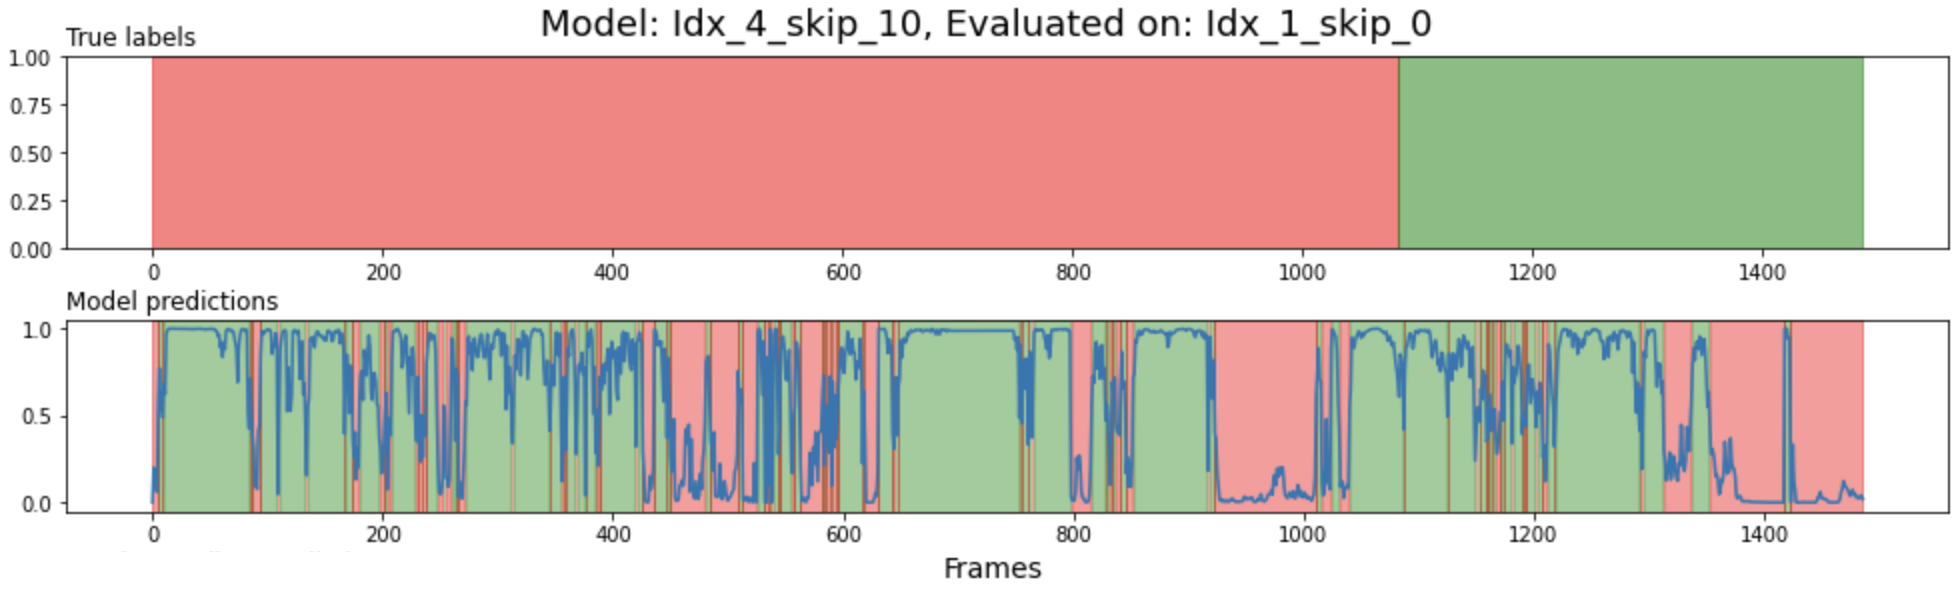
\includegraphics[width=\linewidth]{Materials/Results/SP/M1On1C}
	\end{subfigure}
	\\
	\begin{subfigure}{\linewidth}
		\centering
		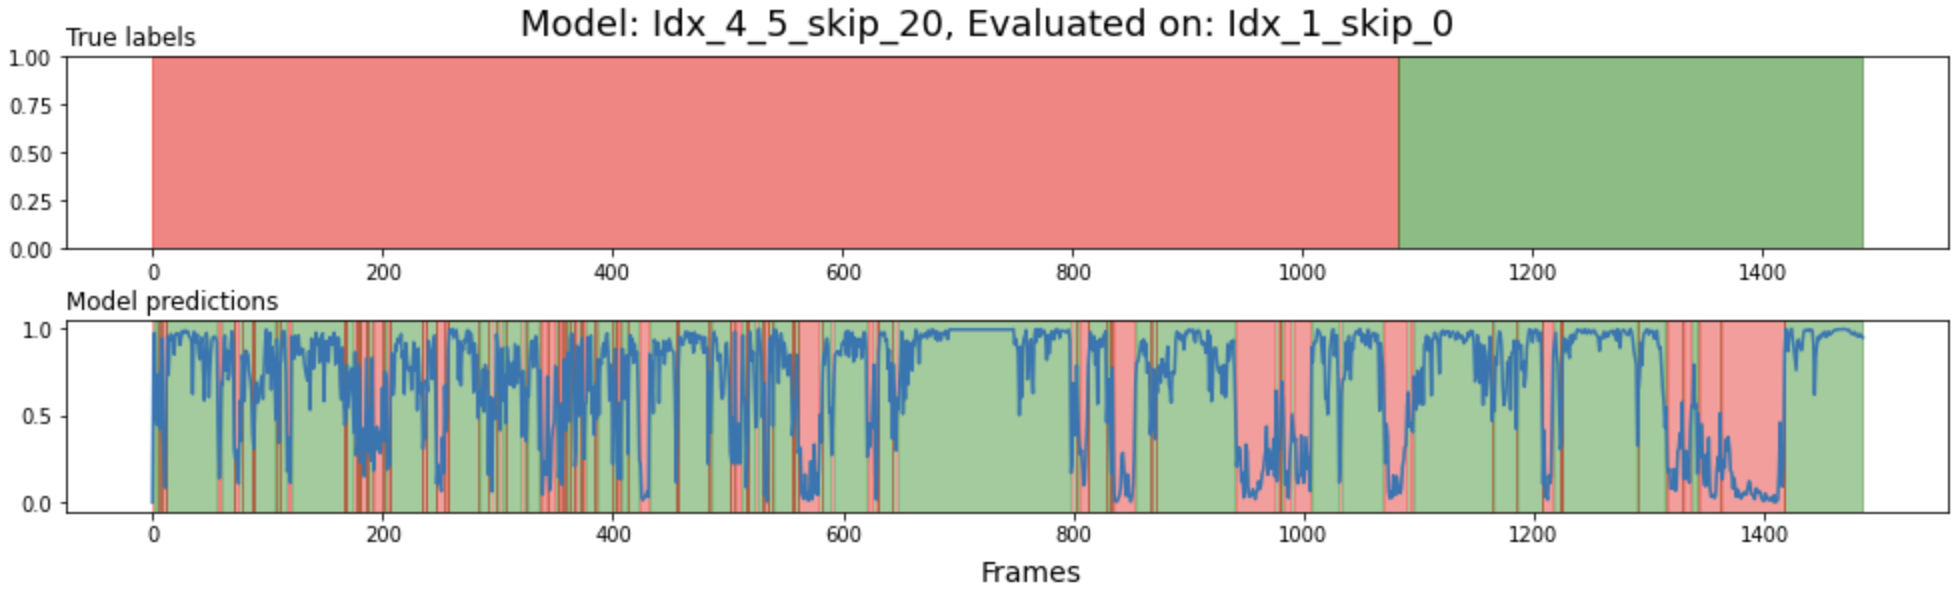
\includegraphics[width=\linewidth]{Materials/Results/SP/M2On1C}
	\end{subfigure}
	\\
	\begin{subfigure}{\linewidth}
		\centering
		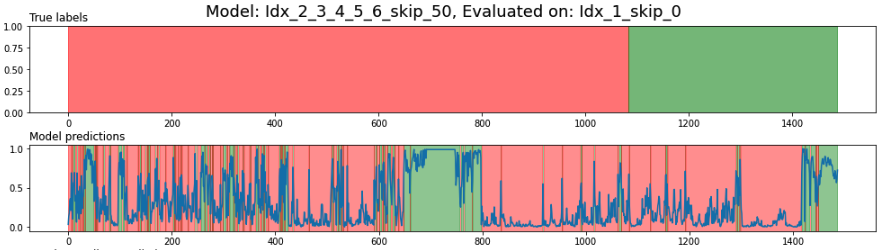
\includegraphics[width=\linewidth]{Materials/Results/SP/M3On1C}
	\end{subfigure}
	\\
	\begin{subfigure}{\linewidth}
		\centering
		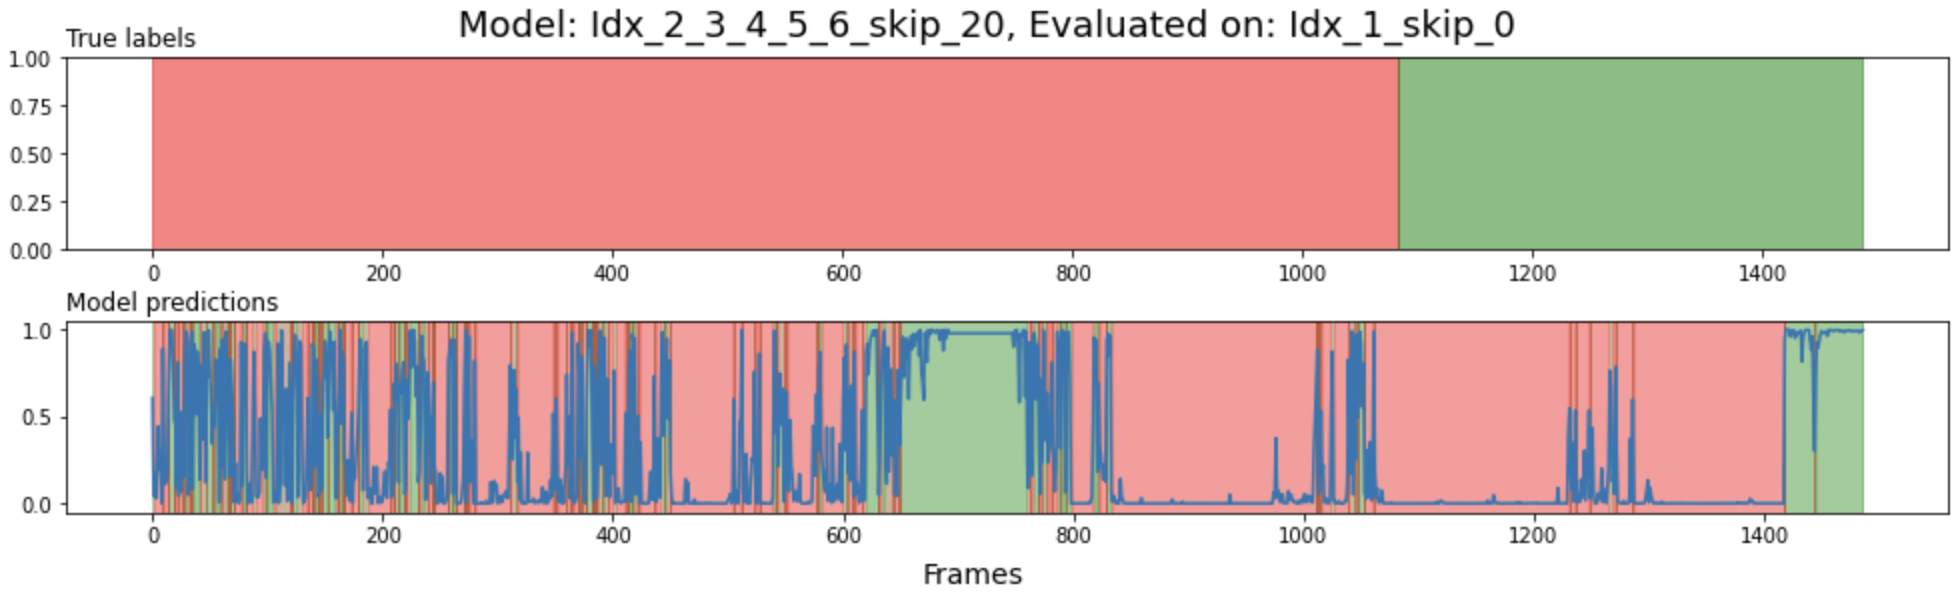
\includegraphics[width=\linewidth]{Materials/Results/SP/M4On1C}
	\end{subfigure}
	\\
	\begin{subfigure}{\linewidth}
		\centering
		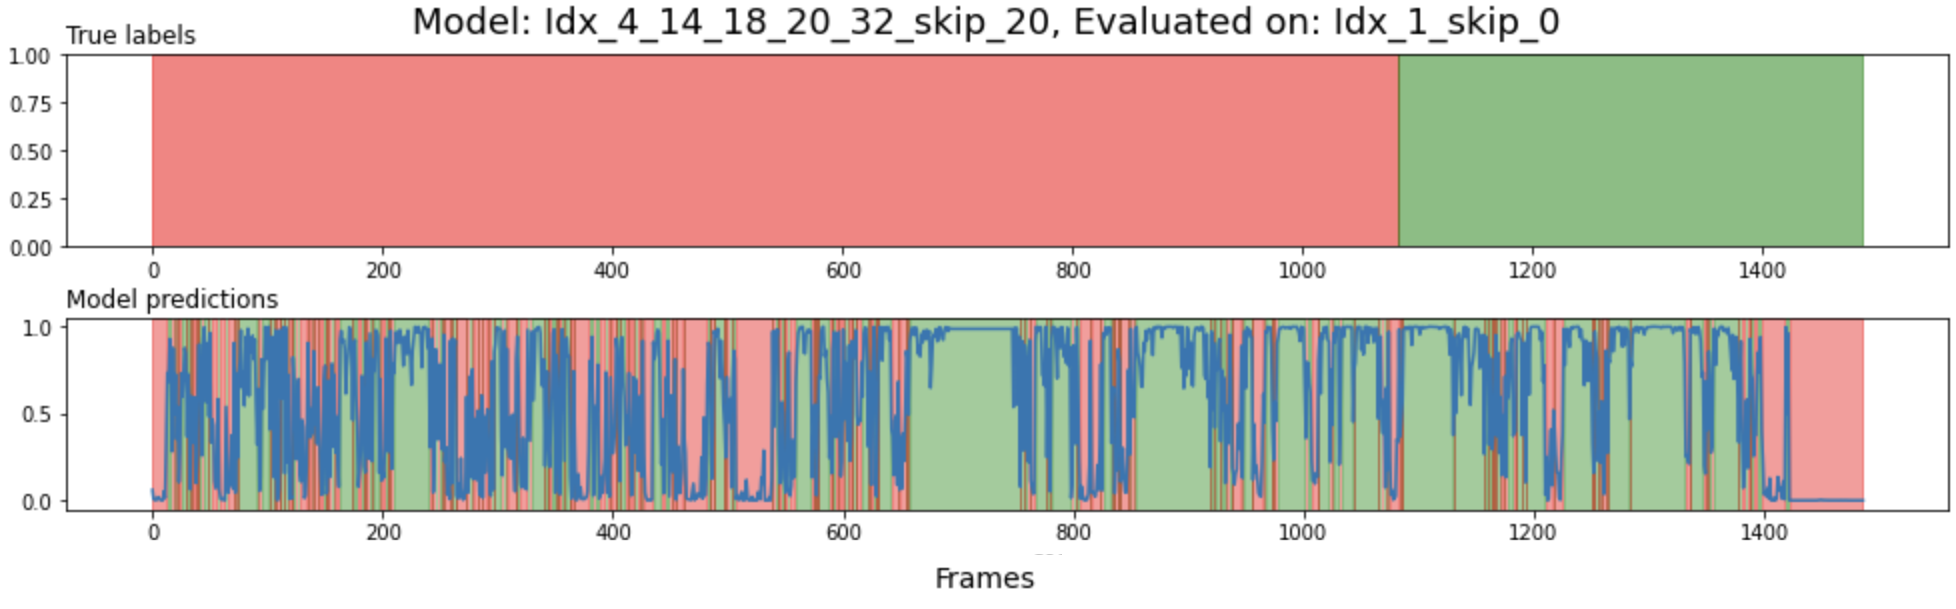
\includegraphics[width=\linewidth]{Materials/Results/SP/M5On1C}
	\end{subfigure}
	\caption{How the first five models predicted on the validation video.}
	\label{firstfive}
\end{figure}

\begin{figure}[H]
	\centering
	\begin{subfigure}{\linewidth}
		\centering
		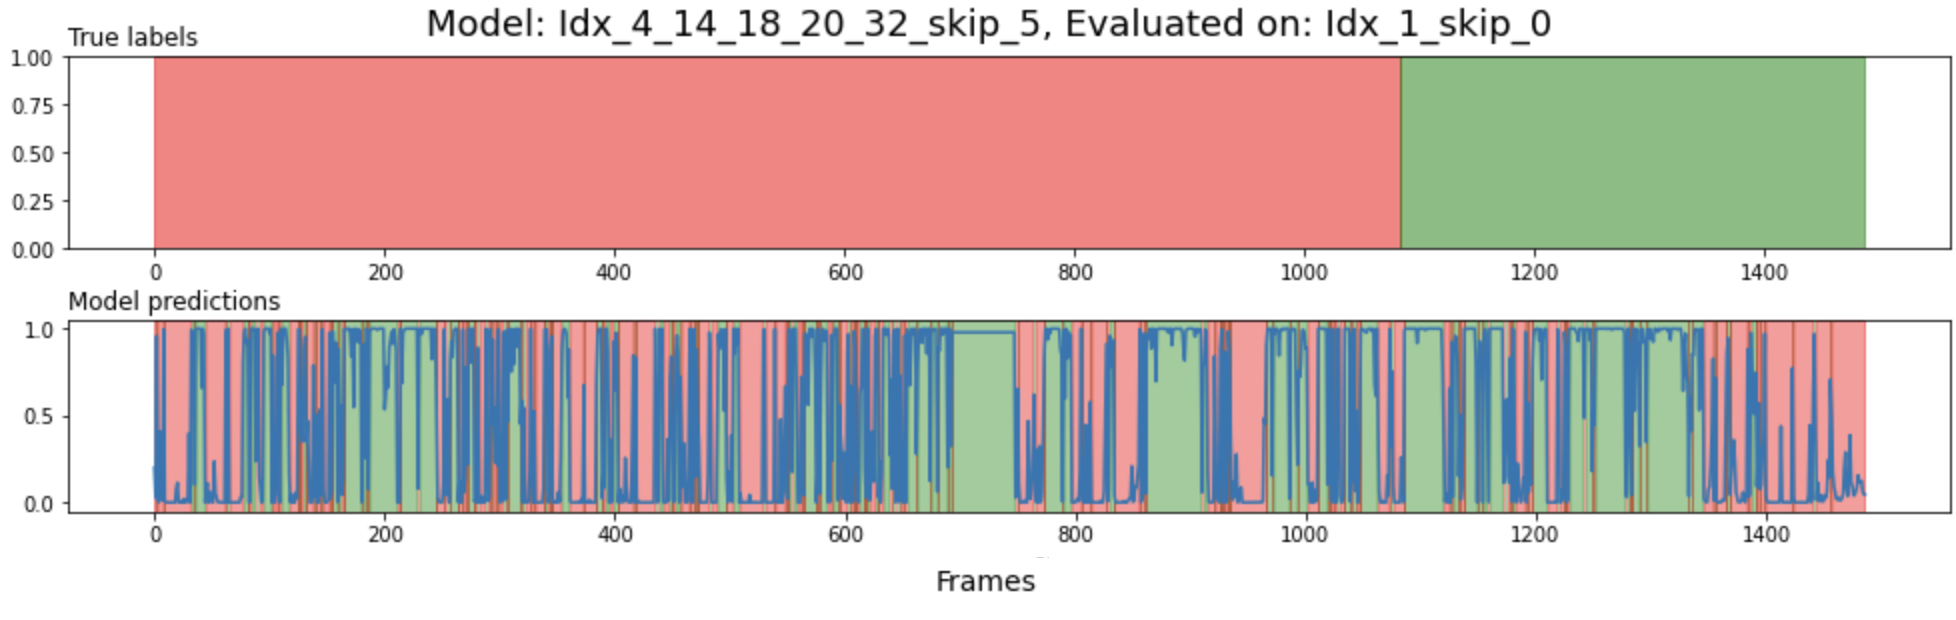
\includegraphics[width=\linewidth]{Materials/Results/SP/M6On1C}
	\end{subfigure}
	\\
	\begin{subfigure}{\linewidth}
		\centering
		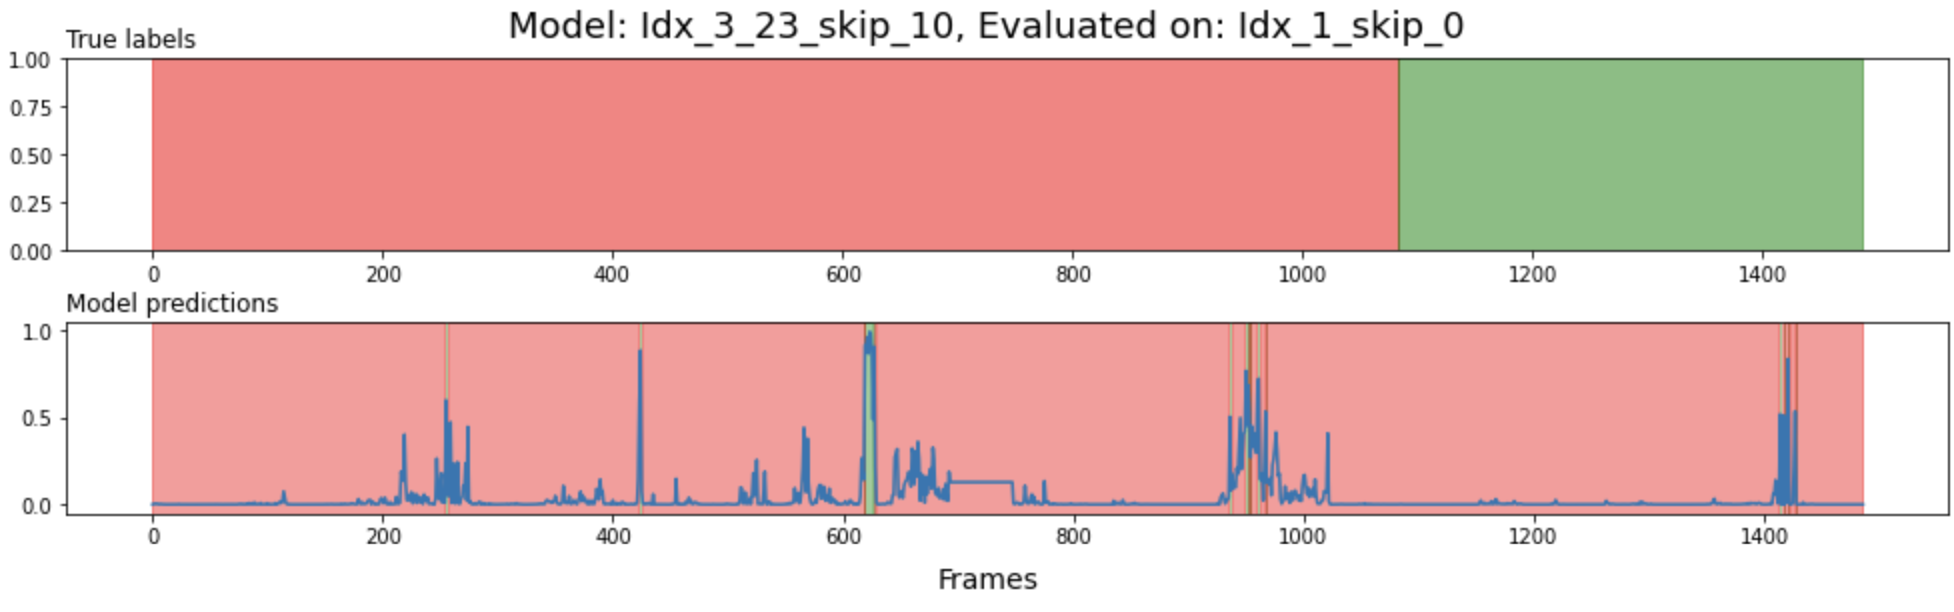
\includegraphics[width=\linewidth]{Materials/Results/SP/M7On1C}
	\end{subfigure}
	\\
	\begin{subfigure}{\linewidth}
		\centering
		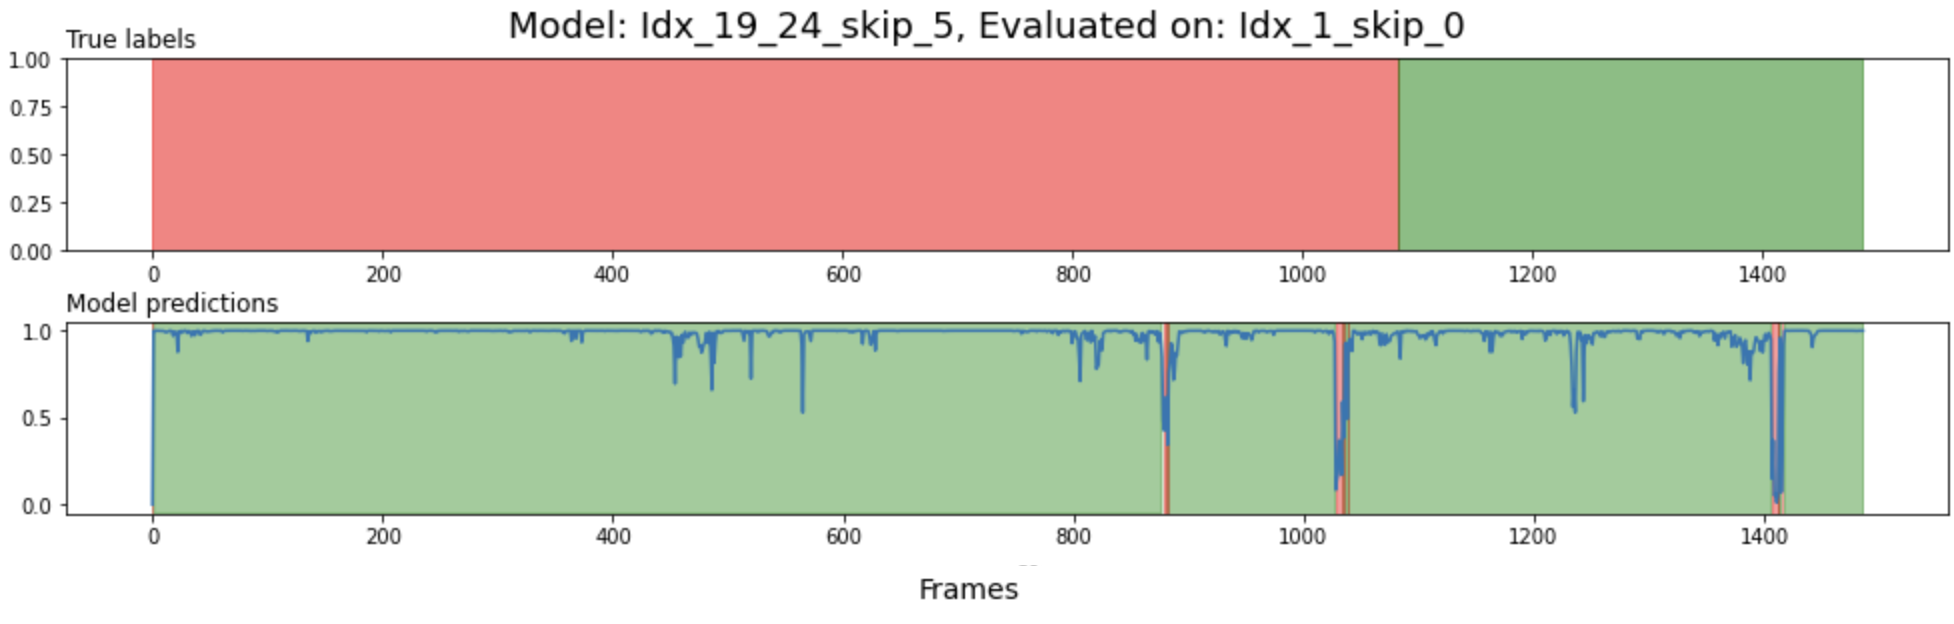
\includegraphics[width=\linewidth]{Materials/Results/SP/M8On1C}
	\end{subfigure}
	\caption{How the last three models predicted on the validation video.}
	\label{lastthree}
\end{figure}

We note how models \textit{Idx\_4\_skip\_10} and \textit{Idx\_4\_5\_skip\_20} predict overly many healthy frames but seem to be fairly confident in their predictions. Model \textit{Idx\_2\_3\_4\_5\_6\_skip\_50} have comparably predicted a lot more inflamed frames, but it still seem to be confident some of the first frames are healthy. Looking at model \textit{Idx\_2\_3\_4\_5\_6\_skip\_20} which scored the second highest validation accuracy, we see it has some rather volatile predictions on the early frames where most however seem to be classified as inflamed. On the other hand, it seem to predict quite confidently too many inflamed frames towards the end of the video. Model \textit{Idx\_4\_14\_18\_20\_32\_skip\_20} is the first model trained across several patients, but this models seem to predict a mix of the previous models as it has some volatile predictions in the beginning of the video, but towards the middle it begins to confidently predict overly many healthy frames. Model \textit{Idx\_4\_14\_18\_20\_32\_skip\_5} is the second model to be trained on several patients and also had a significant larger training set than the other models. Here we see only a few blocks of consecutive healthy predictions and otherwise some very volatile predictions. Towards the end of the video it predicts a large part correctly healthy, but it also predicts the very end inflamed. Model \textit{Idx\_3\_23\_skip\_10} was the model which achieved the highest validation accuracies, but we also see it very rarely predicts other than inflamed. As the validation video

\begin{figure}[H]
	\centering
	\begin{subfigure}{\linewidth}
		\centering
		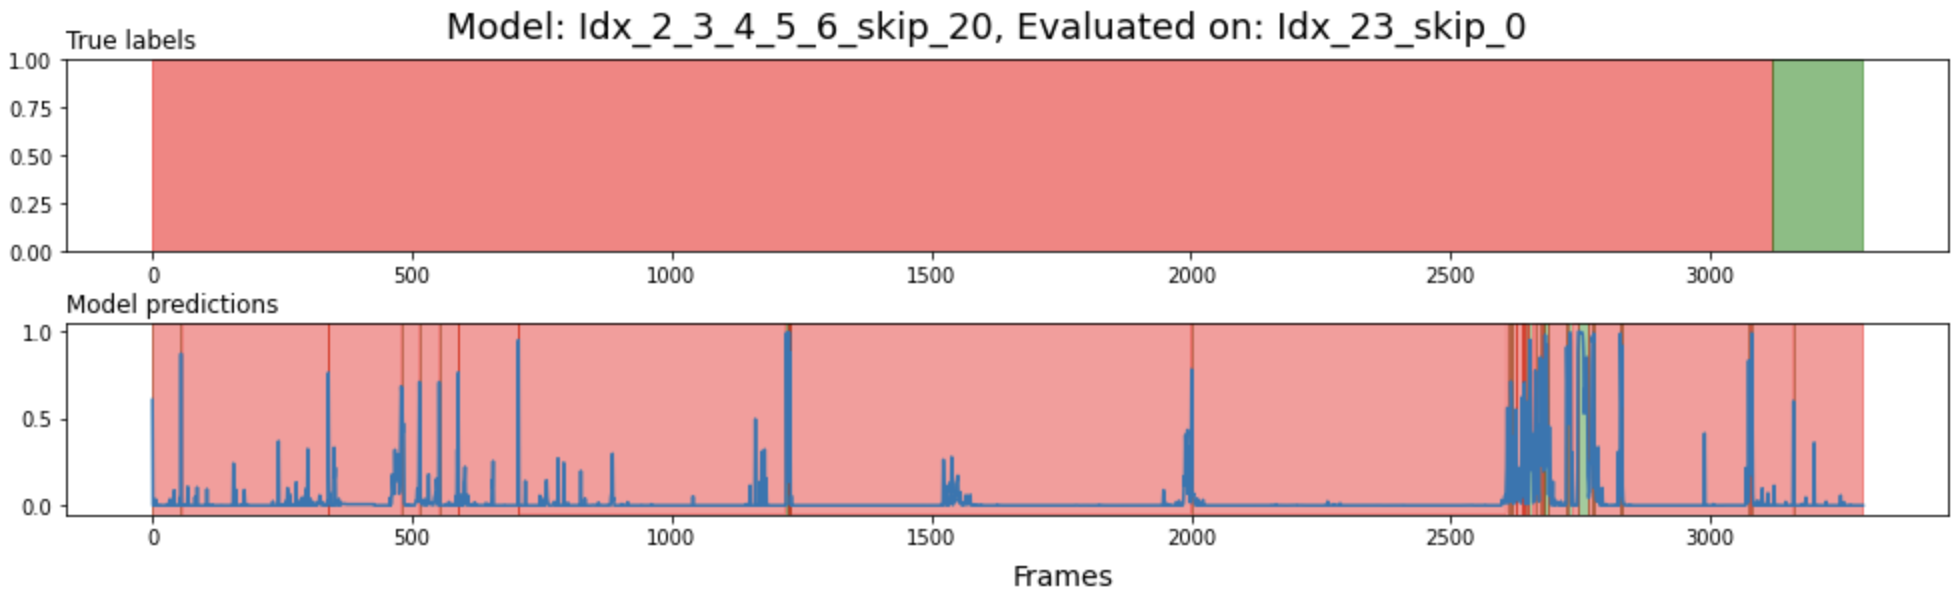
\includegraphics[width=\linewidth]{Materials/Results/SP/M4On23C}
	\end{subfigure}
	\\
	\begin{subfigure}{\linewidth}
		\centering
		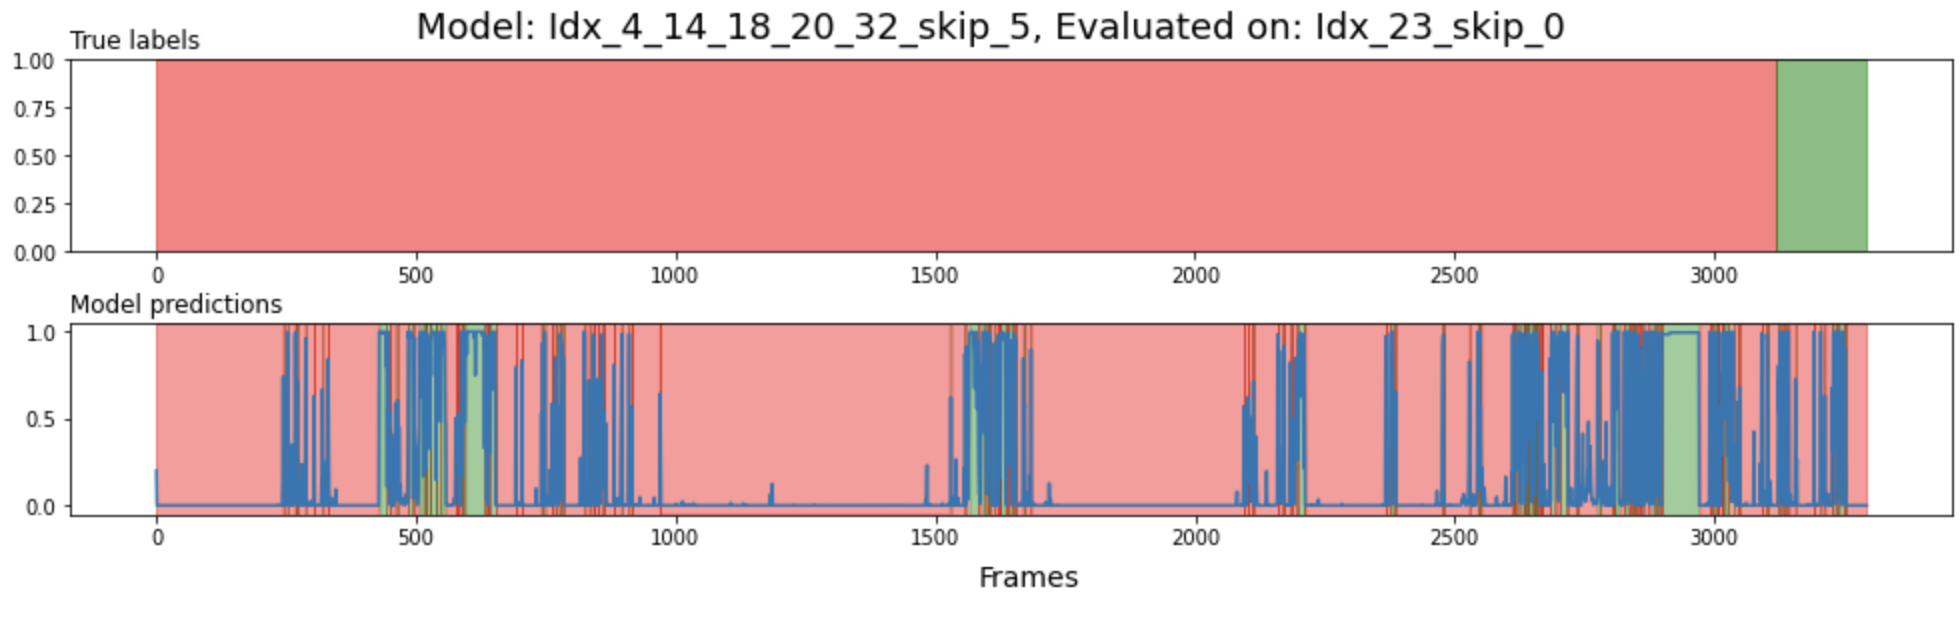
\includegraphics[width=\linewidth]{Materials/Results/SP/M6On23C}
	\end{subfigure}
	\caption{How the two selected models perform on test set \textit{Idx\_23\_skip\_0}.}
	\label{idx23}
\end{figure}

consists of approximately 72\% inflamed frames, it would seem its accuracy is skewed because of the imbalance in the data. Lastly we have model \textit{Idx\_19\_24\_skip\_5} which has the opposite issue where it only predicts healthy.

To select which model to move forward and perform treatment predictions with, models \textit{Idx\_2\_3\_4\_5\_6\_skip\_20} and \textit{Idx\_4\_14\_18\_20\_32\_skip\_5} were selected to predict on more videos. \textit{Idx\_2\_3\_4\_5\_6\_skip\_20} was selected as it seem to predict the best on the validation video and \textit{Idx\_4\_14\_18\_20\_32\_skip\_5} because prior knowledge say models trained on more and varied data should perform better, and thus we verify its validation results from \autoref{2dresnetevalres} are not amiss.

In \autoref{idx23} we see the predictions of the two models on an unseen video which is biased towards being inflamed. We see model \textit{Idx\_2\_3\_4\_5\_6\_skip\_20} predicting confidently and almost exclusively inflammation with a few healthy predictions in the wrong places. Model \textit{Idx\_4\_14\_18\_20\_32\_skip\_5} is more uncertain, and predicts healthy in some spots while having oscillating predictions. The largest consecutive part where it confidently predicts healthy is when it should have predicted inflammation.

In \autoref{idx24} we see the predictions of the two selected models on an unseen video biased towards being healthy. We see model \textit{Idx\_2\_3\_4\_5\_6\_skip\_20} still confidently predicting most frames inflamed, with a few correct exceptions towards the middle of the video. Model \textit{Idx\_4\_14\_18\_20\_32\_skip\_5} predicts most of the video inflamed too, but is not as certain and also correctly predicts one large block healthy.

As a last validation, in \autoref{idx28} we see the predictions of the two selected models on an unseen video biased towards inflammation. Model \textit{Idx\_2\_3\_4\_5\_6\_skip\_20} is rather volatile in its predictions at the beginning of the video, but seem to correctly predict mostly inflammation. Towards the end it seem to capture some of the healthy frames, but predicts a few too many. Model \textit{Idx\_4\_14\_18\_20\_32\_skip\_5} seems on the other hand very volatile, and seem to have some passages where it wrongly predicts healthy. Towards the end we still see some volatile predictions, but it does not seem to capture the healthy frames at the end.

\begin{figure}[H]
	\centering
	\begin{subfigure}{\linewidth}
		\centering
		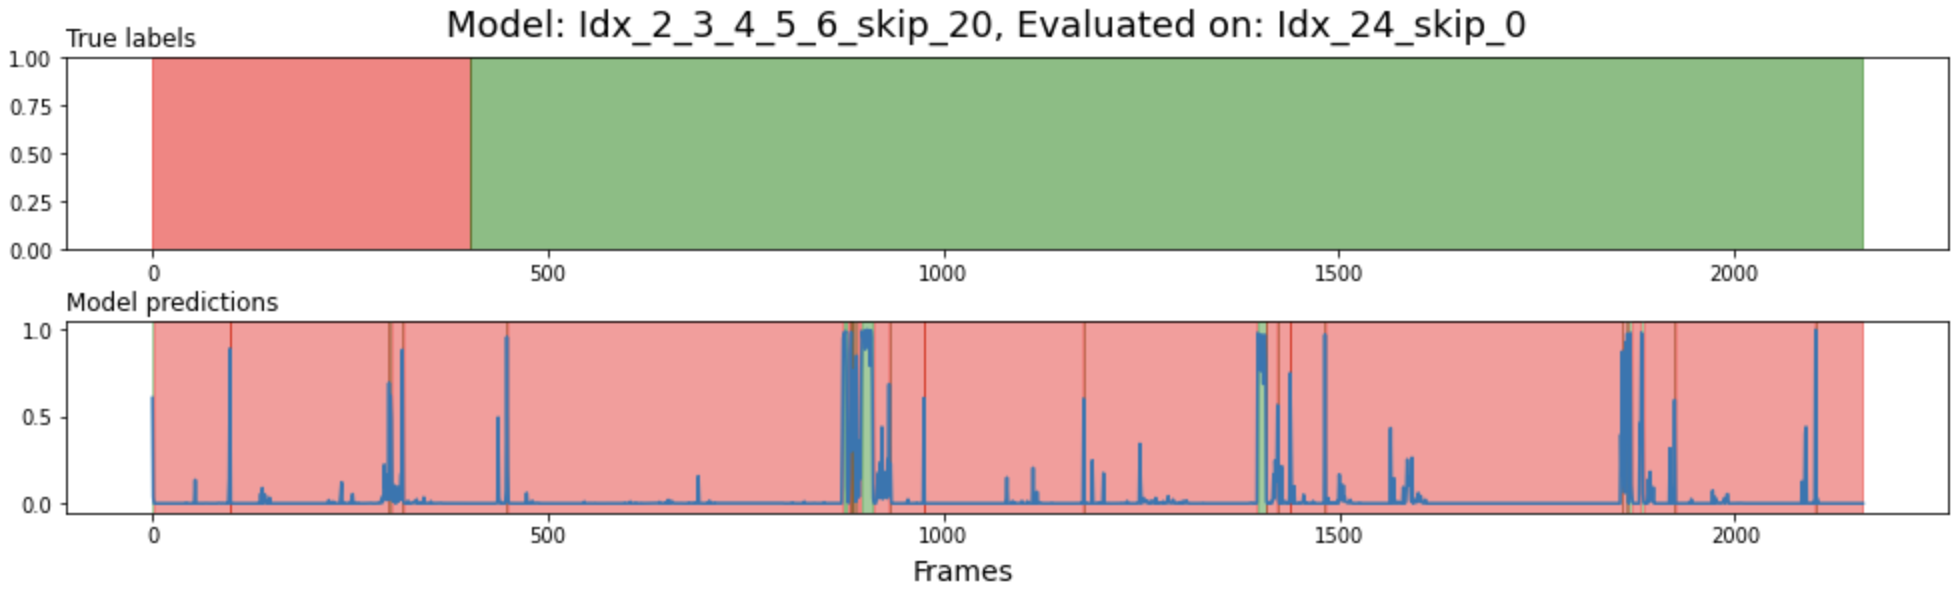
\includegraphics[width=\linewidth]{Materials/Results/SP/M4On24C}
	\end{subfigure}
	\\
	\begin{subfigure}{\linewidth}
		\centering
		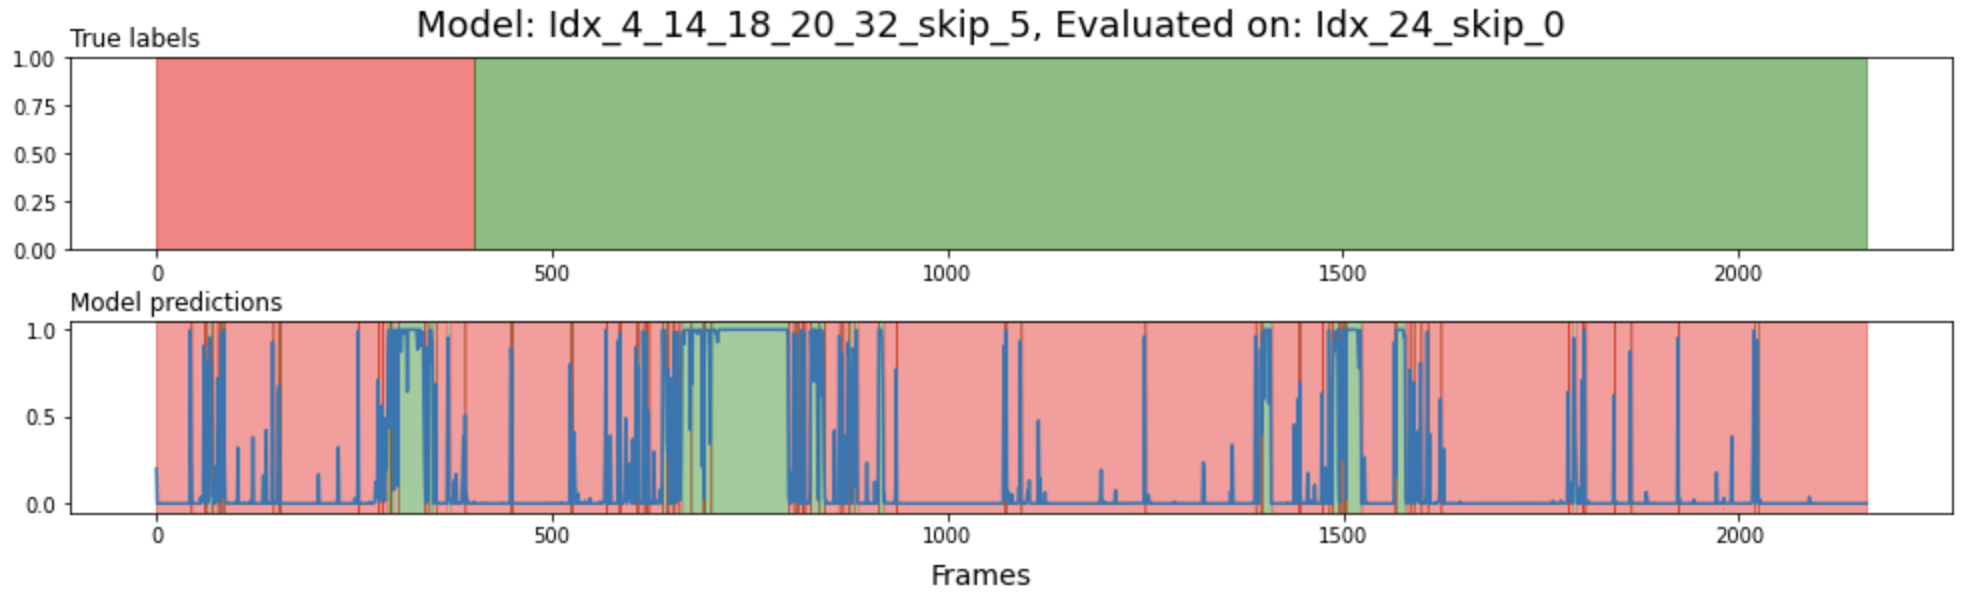
\includegraphics[width=\linewidth]{Materials/Results/SP/M6On24C}
	\end{subfigure}
	\caption{How the two selected models perform on test set \textit{Idx\_24\_skip\_0}.}
	\label{idx24}
\end{figure}

\begin{figure}[H]
	\centering
	\begin{subfigure}{\linewidth}
		\centering
		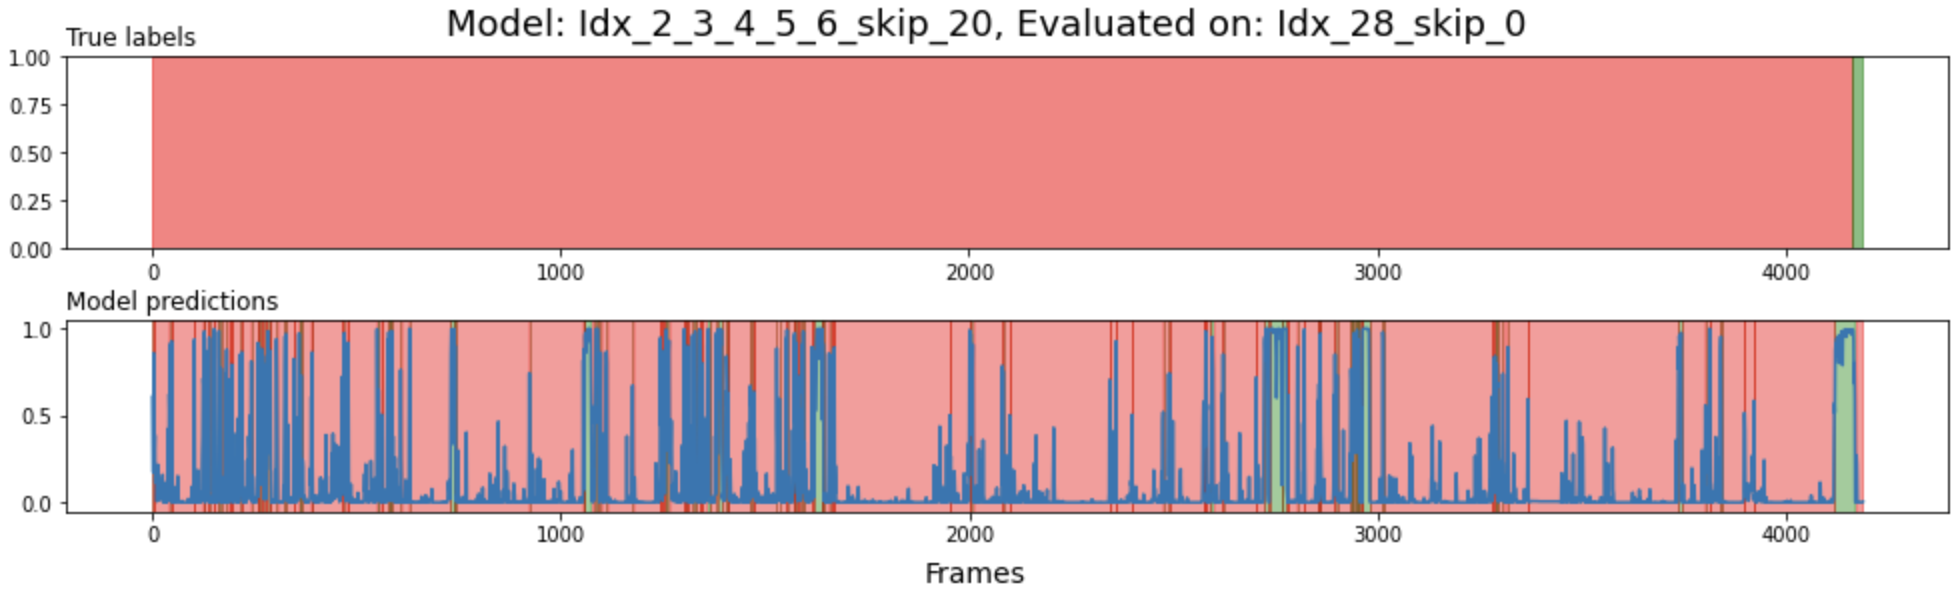
\includegraphics[width=\linewidth]{Materials/Results/SP/M4On28C}
	\end{subfigure}
	\\
	\begin{subfigure}{\linewidth}
		\centering
		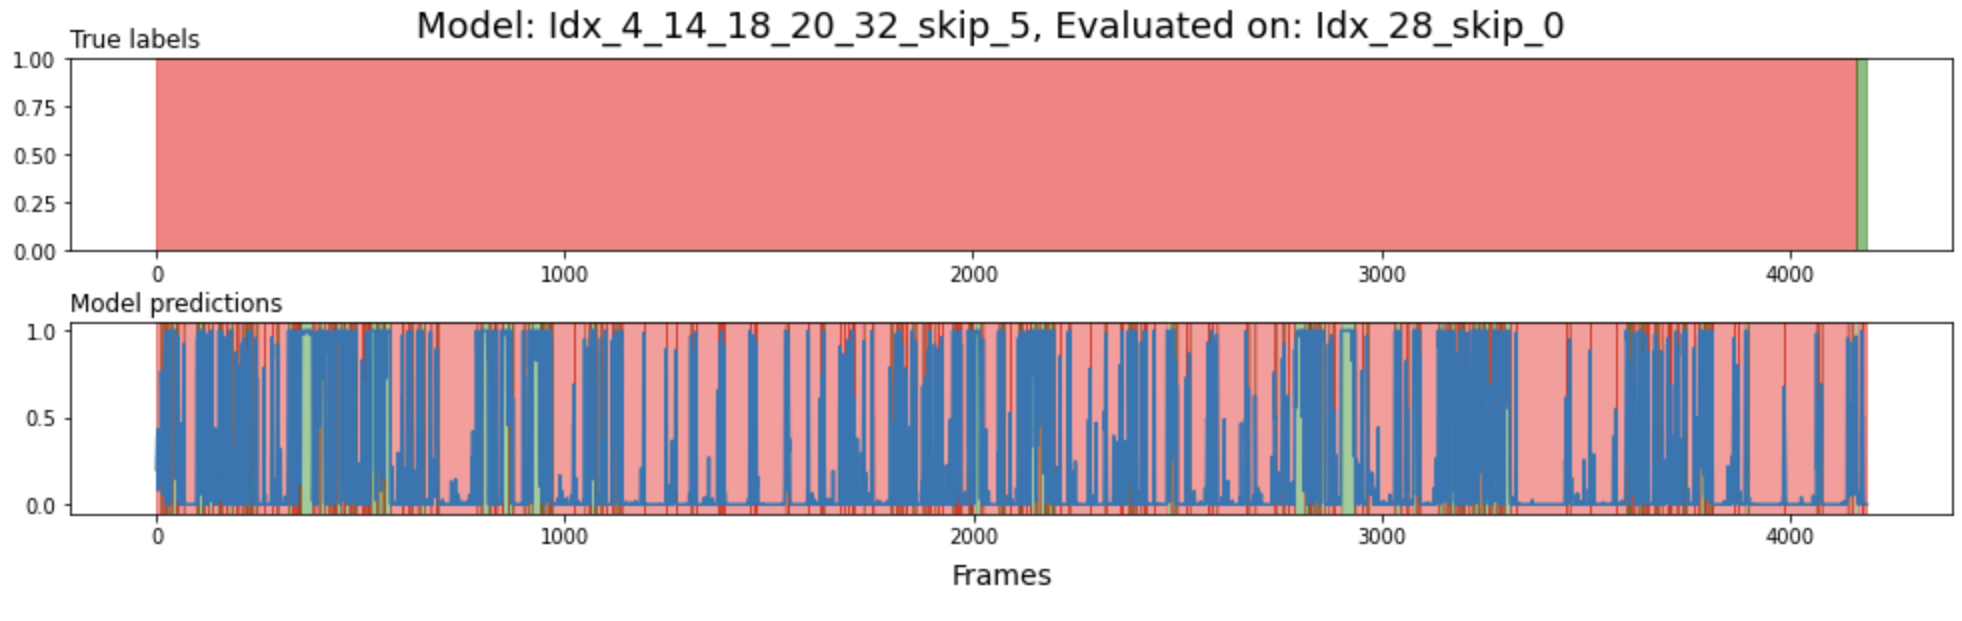
\includegraphics[width=\linewidth]{Materials/Results/SP/M6On28C}
	\end{subfigure}
	\caption{How the two selected models perform on test set \textit{Idx\_28\_skip\_0}.}
	\label{idx28}
\end{figure}

Based on these results model \textit{Idx\_2\_3\_4\_5\_6\_skip\_20} is considered to be the most accurate, and will be used moving forward towards predicting separation points and treatments.
\subsection{Separation point prediction}
Having decided on a model to move forward with, we can now evaluate how well the post-processing approaches performed by looking at their separation point predictions.

\begin{figure}[H]
	\centering
	\begin{subfigure}{\linewidth}
		\centering
		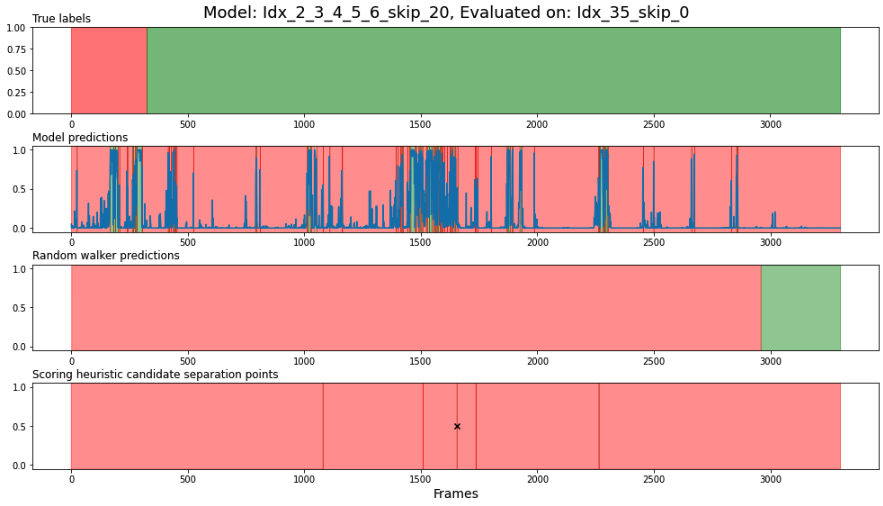
\includegraphics[width=\linewidth]{Materials/Results/SP/M4On35}
	\end{subfigure}
	\\
	\begin{subfigure}{\linewidth}
		\centering
		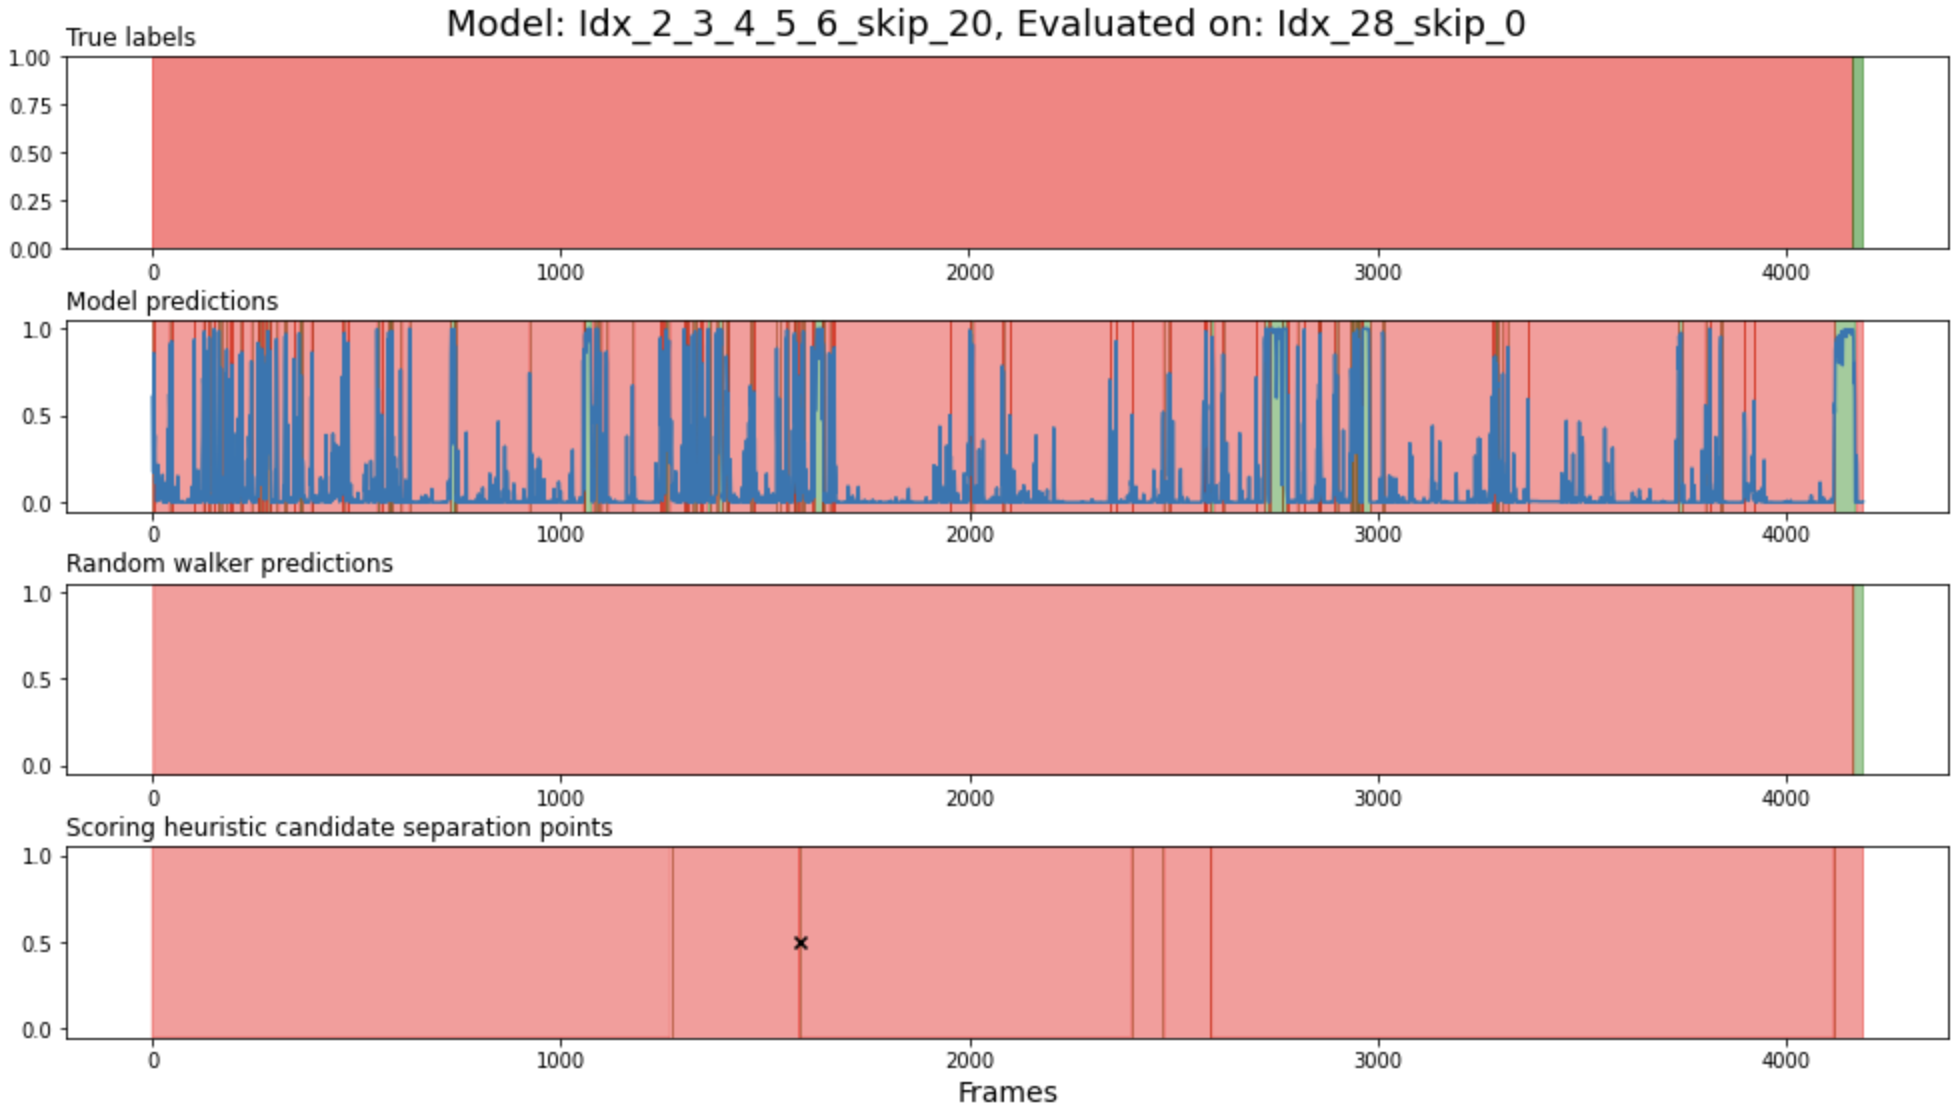
\includegraphics[width=\linewidth]{Materials/Results/SP/M4On28}
	\end{subfigure}
	\caption{Two separation point results.}
	\label{SPRes}
\end{figure}
In \autoref{SPRes} we see two evaluations, each consisting of four bars where the top bar is the true segmentation, the second is model prediction, third is the result of applying the Random Walker post-processing and the fourth is the result of applying the scoring heuristic. It should be noted the scoring heuristic predicts candidate points and one 'believed separation point' marked with an 'x'. This means, the marked points are 'transitions' which has a score less than $0.3$, and the 'x' marks the median of the lowest scoring 'transitions'. The scoring heuristic bar should thus not be read as a segmentation, but as several possible and one believed separation point.

Given the two examples in \autoref{SPRes} we see a tendency for the Random Walker to predict a 'high' separation point, whereas the scoring heuristic is rather insecure due to the insecure model predictions. These are general trends which also can be seen in \autoref{SPTable} where the results for all suitable videos has been reported. Videos 2 through 6 has not been reported as the model was trained on these.\\ 
In \autoref{SPTable} we see the true separation points (row 'True'), the predicted separation points for both post-processing approaches (row 'SH P' and 'RW P'), how far each prediction was from the true separation point measured in absolute number of frames (row 'SH \#' and 'RW \#'), and how far each prediction was measured in percentage of the total number of frames in the video (row 'SH \%' and 'RW \%').

\begin{table}[H]
	\hspace{-1.3cm}
	\begin{tabular}{|c|c|c|c|c|c|c|c|c|c|c|c|c|c|c|c|}
		\hline
		idx   & \multicolumn{1}{c|}{\cellcolor[HTML]{E8E8E8}1}                           & \multicolumn{1}{c|}{\cellcolor[HTML]{E8E8E8}7}                           & \multicolumn{1}{c|}{\cellcolor[HTML]{E8E8E8}8}                           & \multicolumn{1}{c|}{\cellcolor[HTML]{E8E8E8}9}                          & \multicolumn{1}{c|}{\cellcolor[HTML]{E8E8E8}10}                        & \multicolumn{1}{c|}{\cellcolor[HTML]{E8E8E8}11}                        & \multicolumn{1}{c|}{\cellcolor[HTML]{E8E8E8}12}                        & \multicolumn{1}{c|}{\cellcolor[HTML]{E8E8E8}13}                          & \multicolumn{1}{c|}{\cellcolor[HTML]{E8E8E8}14}                          & \multicolumn{1}{c|}{\cellcolor[HTML]{E8E8E8}15}                          & \multicolumn{1}{c|}{\cellcolor[HTML]{E8E8E8}16}                          & \multicolumn{1}{c|}{\cellcolor[HTML]{E8E8E8}17}                          & \multicolumn{1}{c|}{\cellcolor[HTML]{E8E8E8}18}                          & \multicolumn{1}{c|}{\cellcolor[HTML]{E8E8E8}19}                          & \multicolumn{1}{c|}{\cellcolor[HTML]{E8E8E8}20}                          \\ \hline
		True  & \multicolumn{1}{c|}{\cellcolor[HTML]{E8E8E8}{\color[HTML]{000000} 1086}} & \multicolumn{1}{c|}{\cellcolor[HTML]{E8E8E8}{\color[HTML]{000000} 3303}} & \multicolumn{1}{c|}{\cellcolor[HTML]{E8E8E8}{\color[HTML]{000000} 241}}  & \multicolumn{1}{c|}{\cellcolor[HTML]{E8E8E8}{\color[HTML]{000000} 0}}   & \multicolumn{1}{c|}{\cellcolor[HTML]{E8E8E8}{\color[HTML]{000000} 0}}  & \multicolumn{1}{c|}{\cellcolor[HTML]{E8E8E8}{\color[HTML]{000000} 0}}  & \multicolumn{1}{c|}{\cellcolor[HTML]{E8E8E8}{\color[HTML]{000000} 0}}  & \multicolumn{1}{c|}{\cellcolor[HTML]{E8E8E8}{\color[HTML]{000000} 0}}    & \multicolumn{1}{c|}{\cellcolor[HTML]{E8E8E8}{\color[HTML]{000000} 1575}} & \multicolumn{1}{c|}{\cellcolor[HTML]{E8E8E8}{\color[HTML]{000000} 3300}} & \multicolumn{1}{c|}{\cellcolor[HTML]{E8E8E8}{\color[HTML]{000000} 3299}} & \multicolumn{1}{c|}{\cellcolor[HTML]{E8E8E8}{\color[HTML]{000000} 3301}} & \multicolumn{1}{c|}{\cellcolor[HTML]{E8E8E8}{\color[HTML]{000000} 4164}} & \multicolumn{1}{c|}{\cellcolor[HTML]{E8E8E8}{\color[HTML]{000000} 76}}   & \multicolumn{1}{c|}{\cellcolor[HTML]{E8E8E8}{\color[HTML]{000000} 1026}} \\ \hline
		RW P  & \cellcolor[HTML]{ECF4FF}1459                                             & \cellcolor[HTML]{ECF4FF}3279                                             & \cellcolor[HTML]{ECF4FF}202                                              & \cellcolor[HTML]{ECF4FF}4979                                            & \cellcolor[HTML]{ECF4FF}4644                                           & \cellcolor[HTML]{ECF4FF}3300                                           & \cellcolor[HTML]{ECF4FF}3281                                           & \cellcolor[HTML]{ECF4FF}3291                                             & \cellcolor[HTML]{ECF4FF}3291                                             & \cellcolor[HTML]{ECF4FF}3272                                             & \cellcolor[HTML]{ECF4FF}3260                                             & \cellcolor[HTML]{ECF4FF}3255                                             & \cellcolor[HTML]{ECF4FF}4167                                             & \cellcolor[HTML]{ECF4FF}803                                              & \cellcolor[HTML]{ECF4FF}2739                                             \\ \hline
		SH P  & \cellcolor[HTML]{CBCEFB}43                                               & \cellcolor[HTML]{CBCEFB}2345                                             & \cellcolor[HTML]{CBCEFB}107                                              & \cellcolor[HTML]{CBCEFB}614                                             & \cellcolor[HTML]{CBCEFB}2076                                           & \cellcolor[HTML]{CBCEFB}2895                                           & \cellcolor[HTML]{CBCEFB}1354                                           & \cellcolor[HTML]{CBCEFB}3179                                             & \cellcolor[HTML]{CBCEFB}3179                                             & \cellcolor[HTML]{CBCEFB}887                                              & \cellcolor[HTML]{CBCEFB}572                                              & \cellcolor[HTML]{CBCEFB}1400                                             & \cellcolor[HTML]{CBCEFB}4153                                             & \cellcolor[HTML]{CBCEFB}374                                              & \cellcolor[HTML]{CBCEFB}444                                              \\ \hline
		RW \# & \cellcolor[HTML]{ECF4FF}373                                              & \cellcolor[HTML]{ECF4FF}24                                               & \cellcolor[HTML]{ECF4FF}39                                               & \cellcolor[HTML]{ECF4FF}4979                                            & \cellcolor[HTML]{ECF4FF}4644                                           & \cellcolor[HTML]{ECF4FF}3300                                           & \cellcolor[HTML]{ECF4FF}3281                                           & \cellcolor[HTML]{ECF4FF}3291                                             & \cellcolor[HTML]{ECF4FF}1716                                             & \cellcolor[HTML]{ECF4FF}28                                               & \cellcolor[HTML]{ECF4FF}39                                               & \cellcolor[HTML]{ECF4FF}46                                               & \cellcolor[HTML]{ECF4FF}3                                                & \cellcolor[HTML]{ECF4FF}727                                              & \cellcolor[HTML]{ECF4FF}1713                                             \\ \hline
		SH \# & \cellcolor[HTML]{CBCEFB}1043                                             & \cellcolor[HTML]{CBCEFB}958                                              & \cellcolor[HTML]{CBCEFB}134                                              & \cellcolor[HTML]{CBCEFB}614                                             & \cellcolor[HTML]{CBCEFB}2076                                           & \cellcolor[HTML]{CBCEFB}2895                                           & \cellcolor[HTML]{CBCEFB}1354                                           & \cellcolor[HTML]{CBCEFB}3179                                             & \cellcolor[HTML]{CBCEFB}1604                                             & \cellcolor[HTML]{CBCEFB}2413                                             & \cellcolor[HTML]{CBCEFB}2727                                             & \cellcolor[HTML]{CBCEFB}1901                                             & \cellcolor[HTML]{CBCEFB}11                                               & \cellcolor[HTML]{CBCEFB}298                                              & \cellcolor[HTML]{CBCEFB}582                                              \\ \hline
		RW \% & \cellcolor[HTML]{ECF4FF}0.25                                             & \cellcolor[HTML]{ECF4FF}0.01                                             & \cellcolor[HTML]{ECF4FF}0.16                                             & \cellcolor[HTML]{ECF4FF}1.00                                            & \cellcolor[HTML]{ECF4FF}0.93                                           & \cellcolor[HTML]{ECF4FF}0.66                                           & \cellcolor[HTML]{ECF4FF}0.99                                           & \cellcolor[HTML]{ECF4FF}1.00                                             & \cellcolor[HTML]{ECF4FF}0.52                                             & \cellcolor[HTML]{ECF4FF}0.01                                             & \cellcolor[HTML]{ECF4FF}0.01                                             & \cellcolor[HTML]{ECF4FF}0.01                                             & \cellcolor[HTML]{ECF4FF}0.00                                             & \cellcolor[HTML]{ECF4FF}0.87                                             & \cellcolor[HTML]{ECF4FF}0.52                                             \\ \hline
		SH \% & \cellcolor[HTML]{CBCEFB}0.70                                             & \cellcolor[HTML]{CBCEFB}0.29                                             & \cellcolor[HTML]{CBCEFB}0.56                                             & \cellcolor[HTML]{CBCEFB}0.12                                            & \cellcolor[HTML]{CBCEFB}0.42                                           & \cellcolor[HTML]{CBCEFB}0.58                                           & \cellcolor[HTML]{CBCEFB}0.41                                           & \cellcolor[HTML]{CBCEFB}0.96                                             & \cellcolor[HTML]{CBCEFB}0.49                                             & \cellcolor[HTML]{CBCEFB}0.73                                             & \cellcolor[HTML]{CBCEFB}0.83                                             & \cellcolor[HTML]{CBCEFB}0.58                                             & \cellcolor[HTML]{CBCEFB}0.00                                             & \cellcolor[HTML]{CBCEFB}0.36                                             & \cellcolor[HTML]{CBCEFB}0.18                                             \\ \hline\hline
		idx   & \multicolumn{1}{c|}{\cellcolor[HTML]{E8E8E8}{\color[HTML]{000000} 21}}   & \multicolumn{1}{c|}{\cellcolor[HTML]{E8E8E8}{\color[HTML]{000000} 22}}   & \multicolumn{1}{c|}{\cellcolor[HTML]{E8E8E8}{\color[HTML]{000000} 23}}   & \multicolumn{1}{c|}{\cellcolor[HTML]{E8E8E8}{\color[HTML]{000000} 24}}  & \multicolumn{1}{c|}{\cellcolor[HTML]{E8E8E8}{\color[HTML]{000000} 25}} & \multicolumn{1}{c|}{\cellcolor[HTML]{E8E8E8}{\color[HTML]{000000} 26}} & \multicolumn{1}{c|}{\cellcolor[HTML]{E8E8E8}{\color[HTML]{000000} 27}} & \multicolumn{1}{c|}{\cellcolor[HTML]{E8E8E8}{\color[HTML]{000000} 28}}   & \multicolumn{1}{c|}{\cellcolor[HTML]{E8E8E8}{\color[HTML]{000000} 29}}   & \multicolumn{1}{c|}{\cellcolor[HTML]{E8E8E8}{\color[HTML]{000000} 30}}   & \multicolumn{1}{c|}{\cellcolor[HTML]{E8E8E8}{\color[HTML]{000000} 31}}   & \multicolumn{1}{c|}{\cellcolor[HTML]{E8E8E8}{\color[HTML]{000000} 32}}   & \multicolumn{1}{c|}{\cellcolor[HTML]{E8E8E8}{\color[HTML]{000000} 33}}   & \multicolumn{1}{c|}{\cellcolor[HTML]{E8E8E8}{\color[HTML]{000000} 34}}   & \multicolumn{1}{c|}{\cellcolor[HTML]{E8E8E8}{\color[HTML]{000000} 35}}   \\ \hline
		True  & \multicolumn{1}{c|}{\cellcolor[HTML]{E8E8E8}{\color[HTML]{000000} 3295}} & \multicolumn{1}{c|}{\cellcolor[HTML]{E8E8E8}{\color[HTML]{000000} 3299}} & \multicolumn{1}{c|}{\cellcolor[HTML]{E8E8E8}{\color[HTML]{000000} 3119}} & \multicolumn{1}{c|}{\cellcolor[HTML]{E8E8E8}{\color[HTML]{000000} 402}} & \multicolumn{1}{c|}{\cellcolor[HTML]{E8E8E8}{\color[HTML]{000000} 0}}  & \multicolumn{1}{c|}{\cellcolor[HTML]{E8E8E8}{\color[HTML]{000000} 0}}  & \multicolumn{1}{c|}{\cellcolor[HTML]{E8E8E8}{\color[HTML]{000000} 0}}  & \multicolumn{1}{c|}{\cellcolor[HTML]{E8E8E8}{\color[HTML]{000000} 4164}} & \multicolumn{1}{c|}{\cellcolor[HTML]{E8E8E8}{\color[HTML]{000000} 0}}    & \multicolumn{1}{c|}{\cellcolor[HTML]{E8E8E8}{\color[HTML]{000000} 0}}    & \multicolumn{1}{c|}{\cellcolor[HTML]{E8E8E8}{\color[HTML]{000000} 0}}    & \multicolumn{1}{c|}{\cellcolor[HTML]{E8E8E8}{\color[HTML]{000000} 0}}    & \multicolumn{1}{c|}{\cellcolor[HTML]{E8E8E8}{\color[HTML]{000000} 3299}} & \multicolumn{1}{c|}{\cellcolor[HTML]{E8E8E8}{\color[HTML]{000000} 3302}} & \multicolumn{1}{c|}{\cellcolor[HTML]{E8E8E8}{\color[HTML]{000000} 325}}  \\ \hline
		RW P  & \cellcolor[HTML]{ECF4FF}2446                                             & \cellcolor[HTML]{ECF4FF}3261                                             & \cellcolor[HTML]{ECF4FF}3270                                             & \cellcolor[HTML]{ECF4FF}1880                                            & \cellcolor[HTML]{ECF4FF}4978                                           & \cellcolor[HTML]{ECF4FF}4779                                           & \cellcolor[HTML]{ECF4FF}4674                                           & \cellcolor[HTML]{ECF4FF}4167                                             & \cellcolor[HTML]{ECF4FF}49                                               & \cellcolor[HTML]{ECF4FF}3259                                             & \cellcolor[HTML]{ECF4FF}3293                                             & \cellcolor[HTML]{ECF4FF}3261                                             & \cellcolor[HTML]{ECF4FF}3296                                             & \cellcolor[HTML]{ECF4FF}3295                                             & \cellcolor[HTML]{ECF4FF}2958                                             \\ \hline
		SH P  & \cellcolor[HTML]{CBCEFB}2441                                             & \cellcolor[HTML]{CBCEFB}543                                              & \cellcolor[HTML]{CBCEFB}1221                                             & \cellcolor[HTML]{CBCEFB}1428                                            & \cellcolor[HTML]{CBCEFB}1672                                           & \cellcolor[HTML]{CBCEFB}2113                                           & \cellcolor[HTML]{CBCEFB}4672                                           & \cellcolor[HTML]{CBCEFB}4153                                             & \cellcolor[HTML]{CBCEFB}53                                               & \cellcolor[HTML]{CBCEFB}2202                                             & \cellcolor[HTML]{CBCEFB}2586                                             & \cellcolor[HTML]{CBCEFB}3052                                             & \cellcolor[HTML]{CBCEFB}2562                                             & \cellcolor[HTML]{CBCEFB}1614                                             & \cellcolor[HTML]{CBCEFB}1653                                             \\ \hline
		RW \# & \cellcolor[HTML]{ECF4FF}849                                              & \cellcolor[HTML]{ECF4FF}38                                               & \cellcolor[HTML]{ECF4FF}151                                              & \cellcolor[HTML]{ECF4FF}1478                                            & \cellcolor[HTML]{ECF4FF}4978                                           & \cellcolor[HTML]{ECF4FF}4779                                           & \cellcolor[HTML]{ECF4FF}4674                                           & \cellcolor[HTML]{ECF4FF}3                                                & \cellcolor[HTML]{ECF4FF}49                                               & \cellcolor[HTML]{ECF4FF}3259                                             & \cellcolor[HTML]{ECF4FF}3293                                             & \cellcolor[HTML]{ECF4FF}3261                                             & \cellcolor[HTML]{ECF4FF}3                                                & \cellcolor[HTML]{ECF4FF}7                                                & \cellcolor[HTML]{ECF4FF}2633                                             \\ \hline
		SH \# & \cellcolor[HTML]{CBCEFB}854                                              & \cellcolor[HTML]{CBCEFB}2756                                             & \cellcolor[HTML]{CBCEFB}1898                                             & \cellcolor[HTML]{CBCEFB}1026                                            & \cellcolor[HTML]{CBCEFB}1672                                           & \cellcolor[HTML]{CBCEFB}2113                                           & \cellcolor[HTML]{CBCEFB}4672                                           & \cellcolor[HTML]{CBCEFB}11                                               & \cellcolor[HTML]{CBCEFB}53                                               & \cellcolor[HTML]{CBCEFB}2202                                             & \cellcolor[HTML]{CBCEFB}2586                                             & \cellcolor[HTML]{CBCEFB}3052                                             & \cellcolor[HTML]{CBCEFB}737                                              & \cellcolor[HTML]{CBCEFB}1688                                             & \cellcolor[HTML]{CBCEFB}1328                                             \\ \hline
		RW \% & \cellcolor[HTML]{ECF4FF}0.26                                             & \cellcolor[HTML]{ECF4FF}0.01                                             & \cellcolor[HTML]{ECF4FF}0.05                                             & \cellcolor[HTML]{ECF4FF}0.68                                            & \cellcolor[HTML]{ECF4FF}1.00                                           & \cellcolor[HTML]{ECF4FF}0.96                                           & \cellcolor[HTML]{ECF4FF}1.00                                           & \cellcolor[HTML]{ECF4FF}0.00                                             & \cellcolor[HTML]{ECF4FF}0.88                                             & \cellcolor[HTML]{ECF4FF}0.99                                             & \cellcolor[HTML]{ECF4FF}1.00                                             & \cellcolor[HTML]{ECF4FF}0.99                                             & \cellcolor[HTML]{ECF4FF}0.00                                             & \cellcolor[HTML]{ECF4FF}0.00                                             & \cellcolor[HTML]{ECF4FF}0.80                                             \\ \hline
		SH \% & \cellcolor[HTML]{CBCEFB}0.26                                             & \cellcolor[HTML]{CBCEFB}0.84                                             & \cellcolor[HTML]{CBCEFB}0.58                                             & \cellcolor[HTML]{CBCEFB}0.47                                            & \cellcolor[HTML]{CBCEFB}0.34                                           & \cellcolor[HTML]{CBCEFB}0.42                                           & \cellcolor[HTML]{CBCEFB}1.00                                           & \cellcolor[HTML]{CBCEFB}0.00                                             & \cellcolor[HTML]{CBCEFB}0.95                                             & \cellcolor[HTML]{CBCEFB}0.67                                             & \cellcolor[HTML]{CBCEFB}0.78                                             & \cellcolor[HTML]{CBCEFB}0.93                                             & \cellcolor[HTML]{CBCEFB}0.22                                             & \cellcolor[HTML]{CBCEFB}0.51                                             & \cellcolor[HTML]{CBCEFB}0.40                                             \\ \hline
	\end{tabular}
	\caption{Separation point predictions for all suitable videos. Each video has been enumerated and given and index to be identified with. The 'True' row depicts the true separation point. 'RW P' is the separation point predicted by the Random Walker. 'SH P' is the predicted separation point for the scoring heuristic (the believed point). 'RW \#' is the absolute number of frames to the true separation point from the Random Walker prediction. 'SH \#' is the absolute number of frames to the true separation point from the scoring heuristic prediction. 'RW \%' is the number of frames from the Random Walker prediction to the true separation point measured as a percentage of the total number of frames in the video. 'SH \%' is the number of frames from the Scoring heuristic prediction to the true separation point measured as a percentage of the total number of frames in the video.}
	\label{SPTable}
\end{table}
Taking a closer look at the results in \autoref{SPTable}, we see the average distance in frames from predictions to true separation points for the Random Walker approach is $1788.6$ frames, while for the scoring heuristic this is $1614.57$ frames. However, if we compute the distances in percentages of the total number of frames Random Walker comes out with an average of $51.85\%$ and the scoring heuristic with $51.87\%$.\\
Taking a look at the distance between the predictions and true separation points in terms of frames for the Random Walker approach (row 'RW \#') we see a quite large variance, as some of the videos with a lot of inflamed frames are predicted very accurately, while most of the videos with a lot of healthy frames are predicted very poorly. In general we see the Random Walker approach being very conservative, and predicting 'high' separation points.\\
Looking at the distance between the predictions and true separation points for the scoring heuristic (row 'SH \#'), we see a lower variance as the scoring heuristic is more willing to predict lower separation points on the videos with many healthy frames, however, it is not as accurate on the videos with a lot of inflamed frames as the Random Walker approach is.
\subsection{Treatment prediction}
Because only 30 data vectors were available and model \textit{Idx\_2\_3\_4\_5\_6\_skip\_20} was trained on five datasets, only 25 data vectors were available for predicting treatments. Two slightly different approaches of training was thus attempted. First, training was conducted by a 'leave-one-out' strategy where a 1D ResNet was trained on 24 data vectors and tested on the last one, while rotating which data vector was left out, and training a new model for each rotation. In the second approach, the true segmentations was included in training which would give 48 training vectors. The same leave-one-out strategy was deployed, but only the predicted segmentation would be used for testing. Each model was trained for 120 epochs, using cross entropy as loss function and Adam for optimization with a learning rate of $10^{-4}$ and with a weight decay of $0.07$. 

\begin{table}[H]
	\hspace{-2.7cm}
	\begin{tabular}{|c|c|c|c|c|c|c|c|c|c|c|c|c|c|c|c|c|c|c|c|c|c|c|c|c|c|}
		\hline
		Idx&1
		&7
		&8
		&14
		&15
		&16
		&17
		&18
		&19
		&20
		&21
		&22
		&23
		&24
		&25
		&26
		&27
		&28
		&29
		&30
		&31
		&32
		&33
		&34
		&35\\\hline\hline
		Predictions&2
		&0
		&0
		&2
		&2
		&0
		&2
		&2
		&2
		&2
		&2
		&2
		&2
		&2
		&2
		&2
		&2
		&2
		&0
		&0
		&2
		&2
		&0
		&2
		&2\\\hline
		True&1
		&3
		&3
		&4
		&2
		&2
		&2
		&1
		&1
		&2
		&2
		&2
		&2
		&1
		&0
		&0
		&0
		&1
		&0
		&0
		&0
		&0
		&2
		&2
		&2\\\hline
	\end{tabular}
	\caption{Training a model only on the predicted segmentations, we find the following treatment predictions and true treatments shown for each video. The treatment classes are: 0 being 'healthy', 1 being 'local 5-ASA', 2 being 'Oral steroid', 3 being 'IV steroid' and 4 being 'oral 5-ASA'.}
	\label{treatmentTable}
\end{table}


\begin{figure}[H]
	\centering
	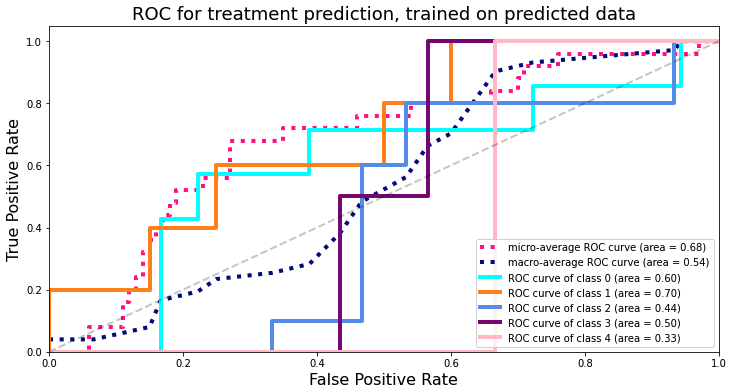
\includegraphics[width=0.85\linewidth]{Materials/Results/Treatment/RocPreds}
	\caption{ROC curves and area under the curve for the five binary 'one-vs-rest' classifiers along with micro- and macro-averages. Training was performed only on predicted segmentations.}
	\label{rocpreds}
\end{figure}
In \autoref{treatmentTable} we see the predicted treatments along the true prescribed treatment, when we train only on predicted segmentations from model \textit{Idx\_2\_3\_4\_5\_6\_skip\_20}. Computing the accuracy of this approach we get $40\%$. However, we note the model only have predicted class 2 and class 0, and there is a heavy class imbalance in the data, with only two examples of class 3 and one example of class 4.\\
It can be hard to assert the quality of a multi class classifier based on accuracy, and thus five binary 'one-vs-rest' classifiers was trained with the same parameters as the original multi class classifier. These binary models was then used to draw ROC curves for which the area under the curves could be computed. The results can be seen in \autoref{rocpreds}.

In \autoref{treatmentTableWithTrue} we see the treatment predictions and true prescribed treatment for each video for a model trained on the predicted segmentations from model \textit{Idx\_2\_3\_4\_5\_6\_skip\_20} and the true segmentations. This model was trained with the same parameters as the previous treatment prediction model. Computing the accuracy we get $48\%$, but we again note only class 0 and class 2 is predicted.
\begin{table}[H]
	\hspace{-2.7cm}
	\begin{tabular}{|c|c|c|c|c|c|c|c|c|c|c|c|c|c|c|c|c|c|c|c|c|c|c|c|c|c|}
		\hline
		Idx&1
		&7
		&8
		&14
		&15
		&16
		&17
		&18
		&19
		&20
		&21
		&22
		&23
		&24
		&25
		&26
		&27
		&28
		&29
		&30
		&31
		&32
		&33
		&34
		&35\\\hline\hline
		Predictions&2
		&0
		&0
		&2
		&2
		&2
		&2
		&2
		&2
		&2
		&2
		&2
		&2
		&2
		&2
		&2
		&2
		&2
		&0
		&0
		&2
		&0
		&0
		&2
		&2\\\hline
		True&1
		&3
		&3
		&4
		&2
		&2
		&2
		&1
		&1
		&2
		&2
		&2
		&2
		&1
		&0
		&0
		&0
		&1
		&0
		&0
		&0
		&0
		&2
		&2
		&2\\\hline
	\end{tabular}
	\caption{Training a model on both the predicted segmentations and true segmentations, we find the following treatment predictions and true treatments shown for each video. The treatment classes are: 0 being 'healthy', 1 being 'local 5-ASA', 2 being 'Oral steroid', 3 being 'IV steroid' and 4 being 'oral 5-ASA'.}
	\label{treatmentTableWithTrue}
\end{table}

In \autoref{rocpredsandtrue} ROC curves are drawn for each of the five binary 'one-vs-rest' classifiers, trained with the same parameters as the original multi class classifier and trained on both predicted and true segmentations.

\begin{figure}[H]
	\centering
	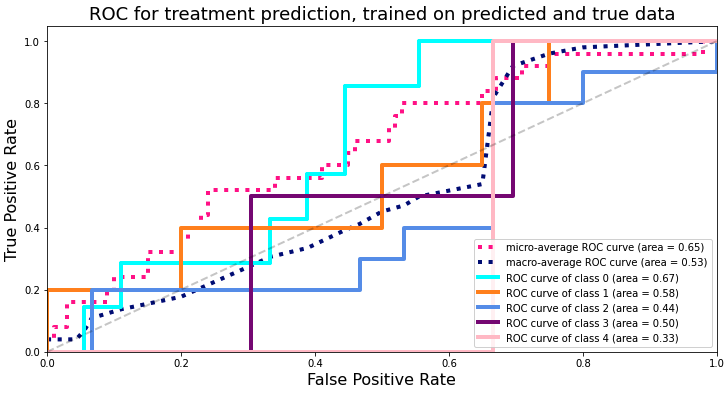
\includegraphics[width=0.85\linewidth]{Materials/Results/Treatment/RocPredsAndTrue}
	\caption{ROC curves and area under the curve for the five binary 'one-vs-rest' classifiers along with micro- and macro-averages. Training was performed on both predicted and true segmentations.}
	\label{rocpredsandtrue}
\end{figure}
\subsection{U-Net for video segmentation}
In an attempt to make the predicted video segmentations from the 2D ResNet model more structured, a 1D U-Net was trained on the predictions of model \textit{Idx\_2\_3\_4\_5\_6\_skip\_20}. Training was conducted in a 'leave-one-out' fashion on the 25 predicted segmentations suitable for treatment predictions. The model was trained for 100 epochs with a learning rate of $3\cdot 10^{-6}$, binary cross entropy as loss function, Adam for optimization and $0.25$ weight decay.\\
The true segmentations was used as target, and was 'artificially' constructed by concatenating a vector of zeros equal in length to the number of frames up to the true separation point, and a vector of ones equal in length to the remaining frames of the video, such that we get one continuous block of inflammation predictions followed by one continuous block of healthy predictions which correspond to how the doctor annotated the video.\\
In the following, four predictions will be reported to show the effect of the trained U-Net model. In each illustration the true segmentation will be shown as the top bar, the 2D ResNet prediction will be shown as the second bar, and the 1D U-Net prediction and its confidence in a healthy prediction will be shown as the third bar.

\begin{figure}[H]
	\centering
	\begin{subfigure}{\linewidth}
		\centering
		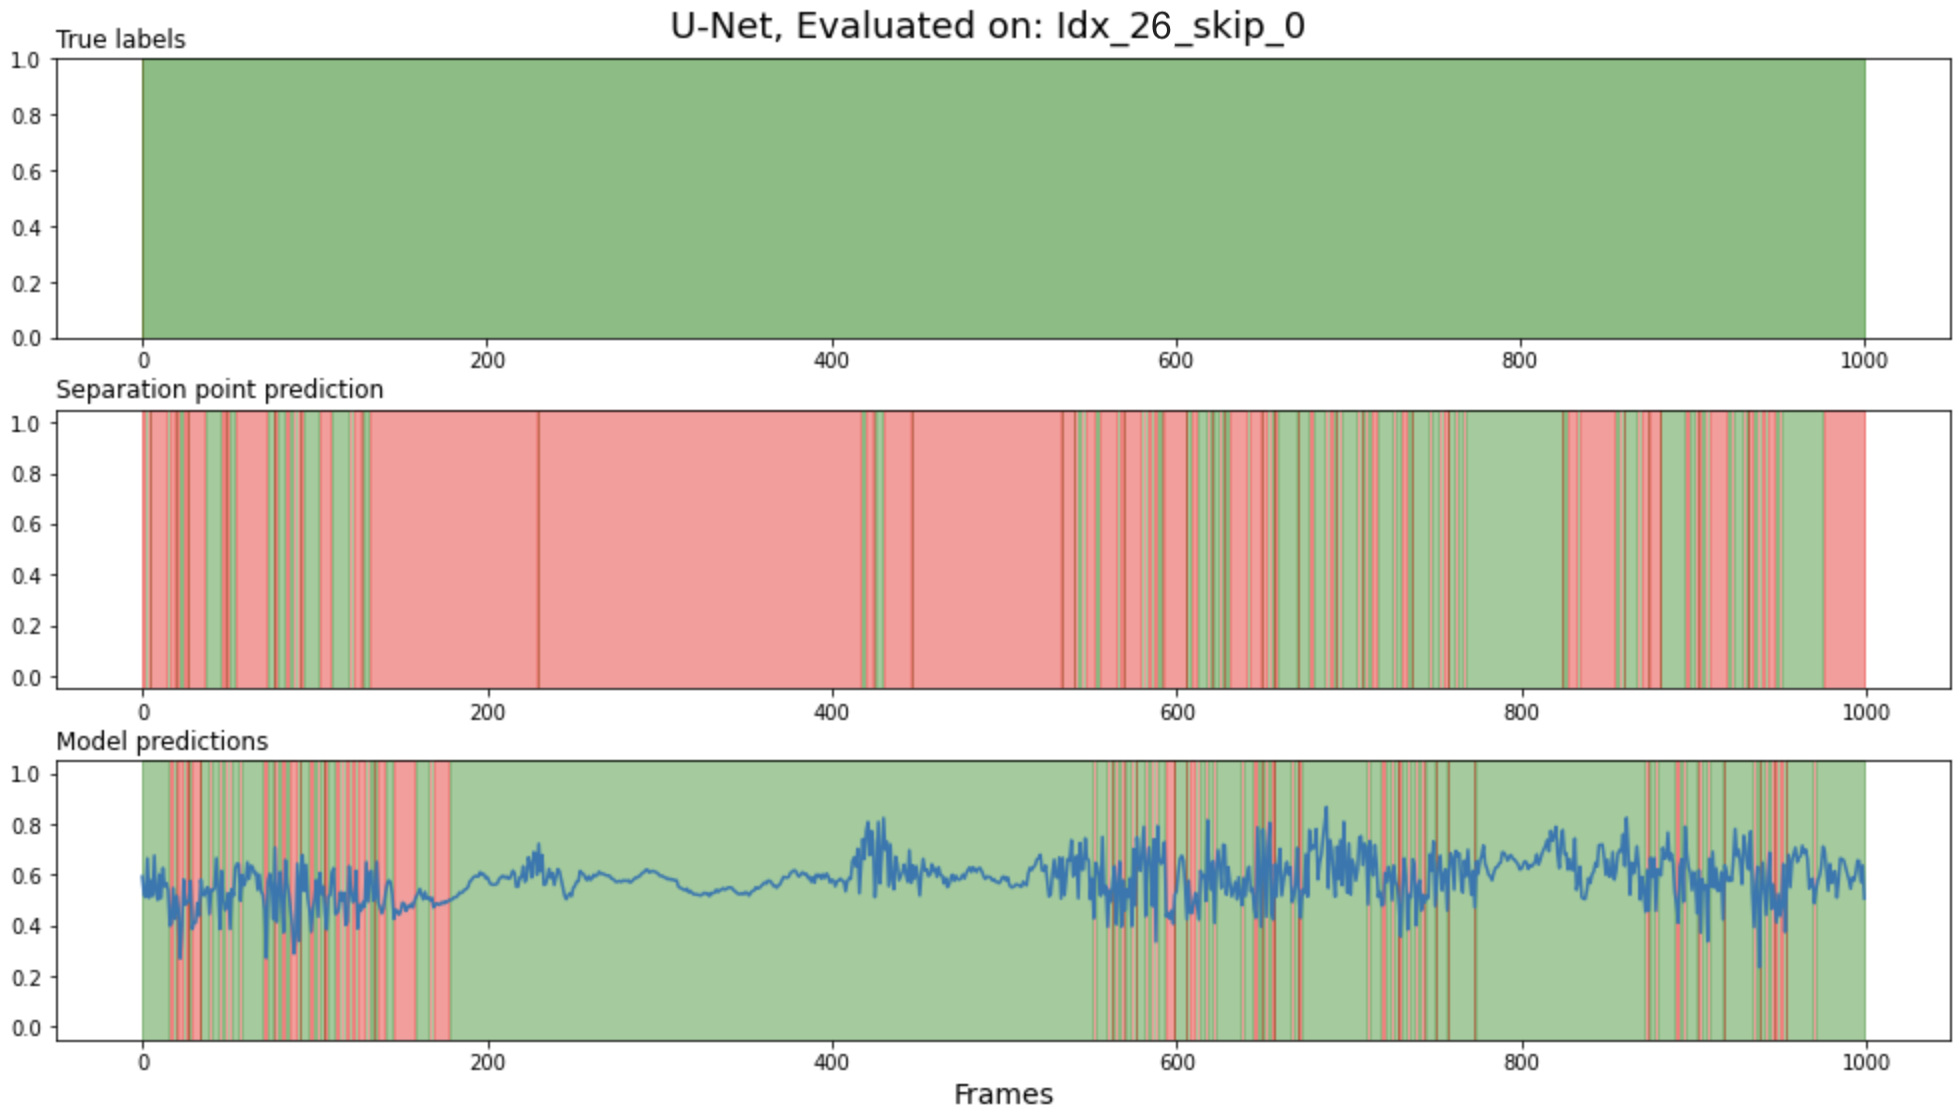
\includegraphics[width=\linewidth]{Materials/Results/UNet/unet1}
	\end{subfigure}
	\\
	\begin{subfigure}{\linewidth}
		\centering
		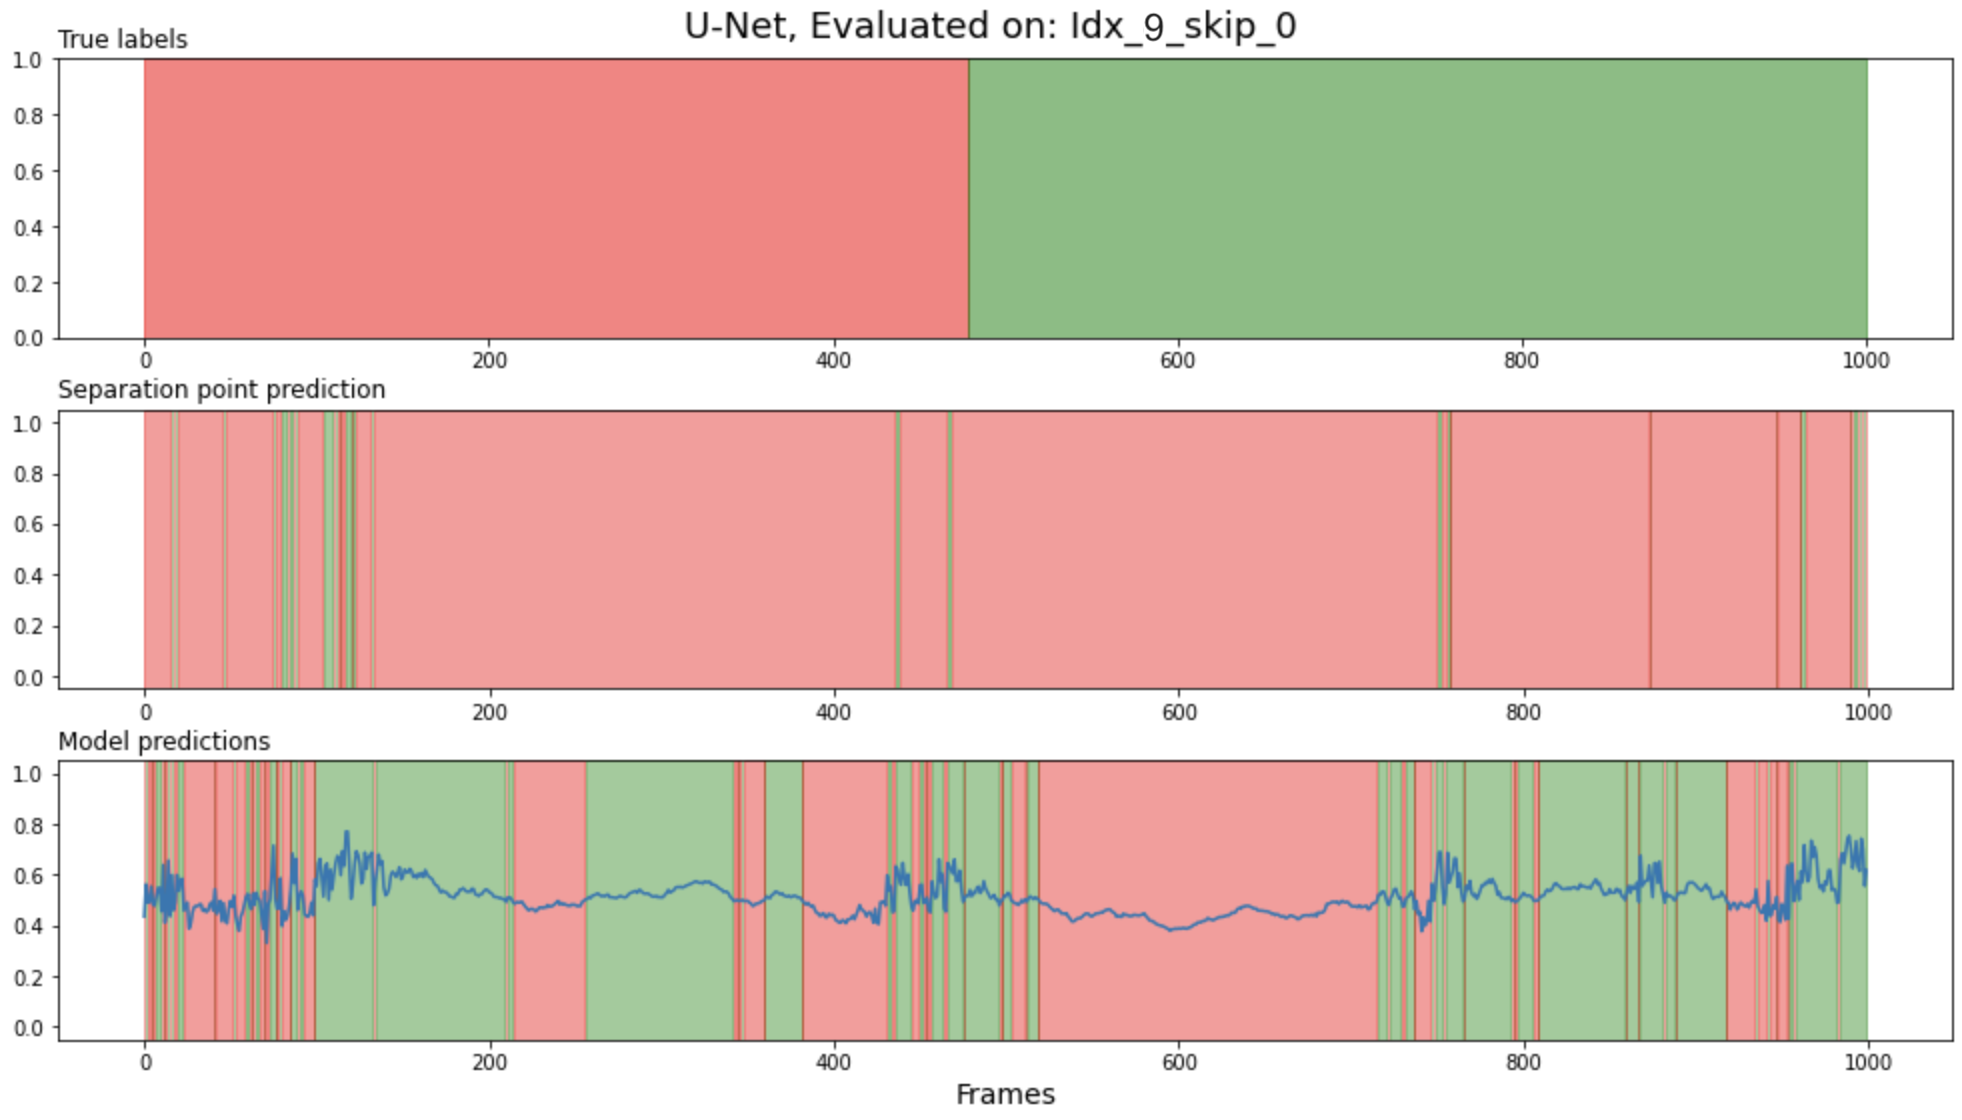
\includegraphics[width=\linewidth]{Materials/Results/UNet/unet2}
	\end{subfigure}
	\caption{Results of 1D U-Net model.}
	\label{unetres1}
\end{figure}

Taking a look at the first result presented in \autoref{unetres1}, we see the true segmentation is all healthy, but the ResNet prediction has a lot of inflammation predictions. Although the U-Net model is not confident in its predictions, it is certain in the sense it does not have very big oscillations. We also see the U-Net predictions have overturned a lot of the inflammation predictions, and made the prediction a lot more representative to the true segmentation.\\
Looking at the second prediction in \autoref{unetres1}, we see the true segmentation being almost half inflammation and half healthy. The ResNet predictions are however almost exclusively inflammation. Again we see the U-Net predictions being very steady and overturning a lot of the inflammation predictions, however this time also making correctly predicted inflamed frames healthy.

\begin{figure}[H]
	\centering
	\begin{subfigure}{\linewidth}
		\centering
		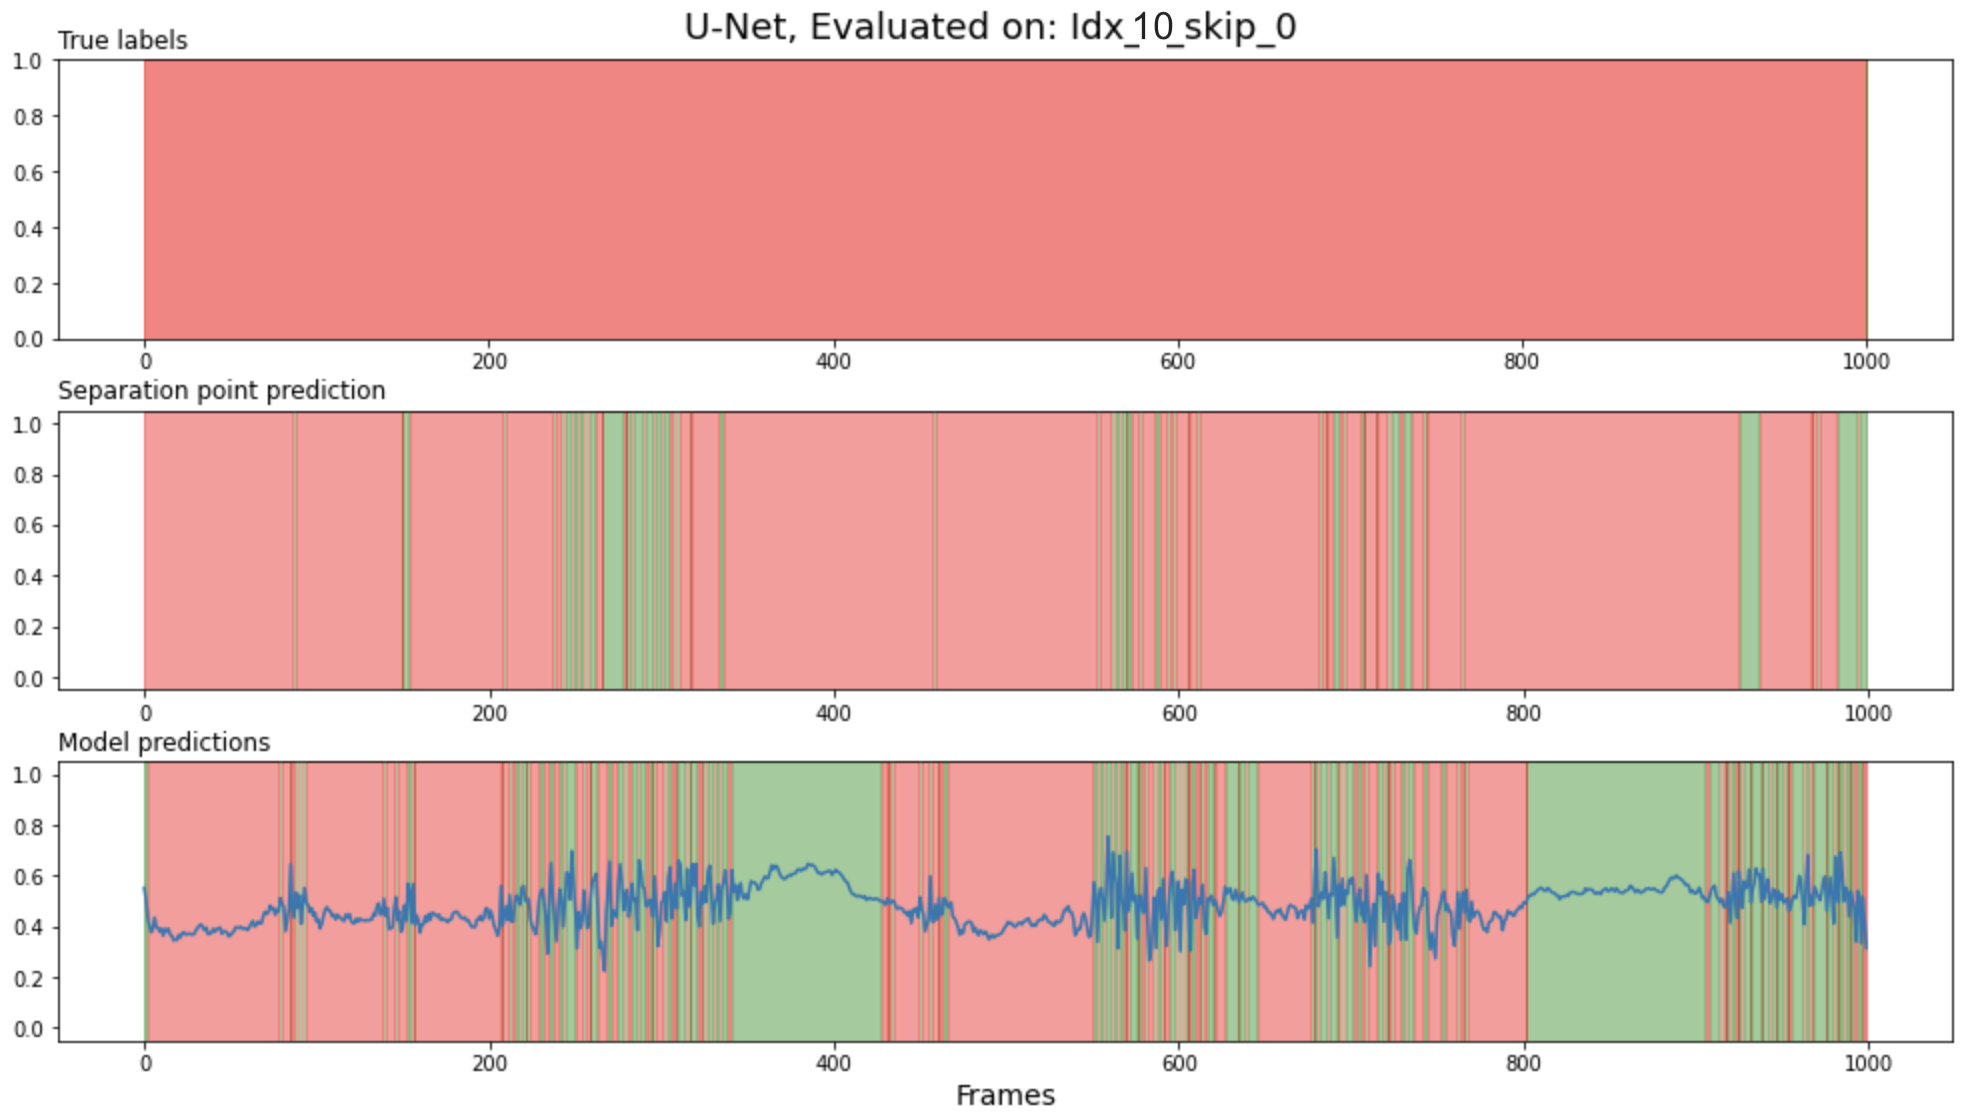
\includegraphics[width=\linewidth]{Materials/Results/UNet/unet3}
	\end{subfigure}
	\\
	\begin{subfigure}{\linewidth}
		\centering
		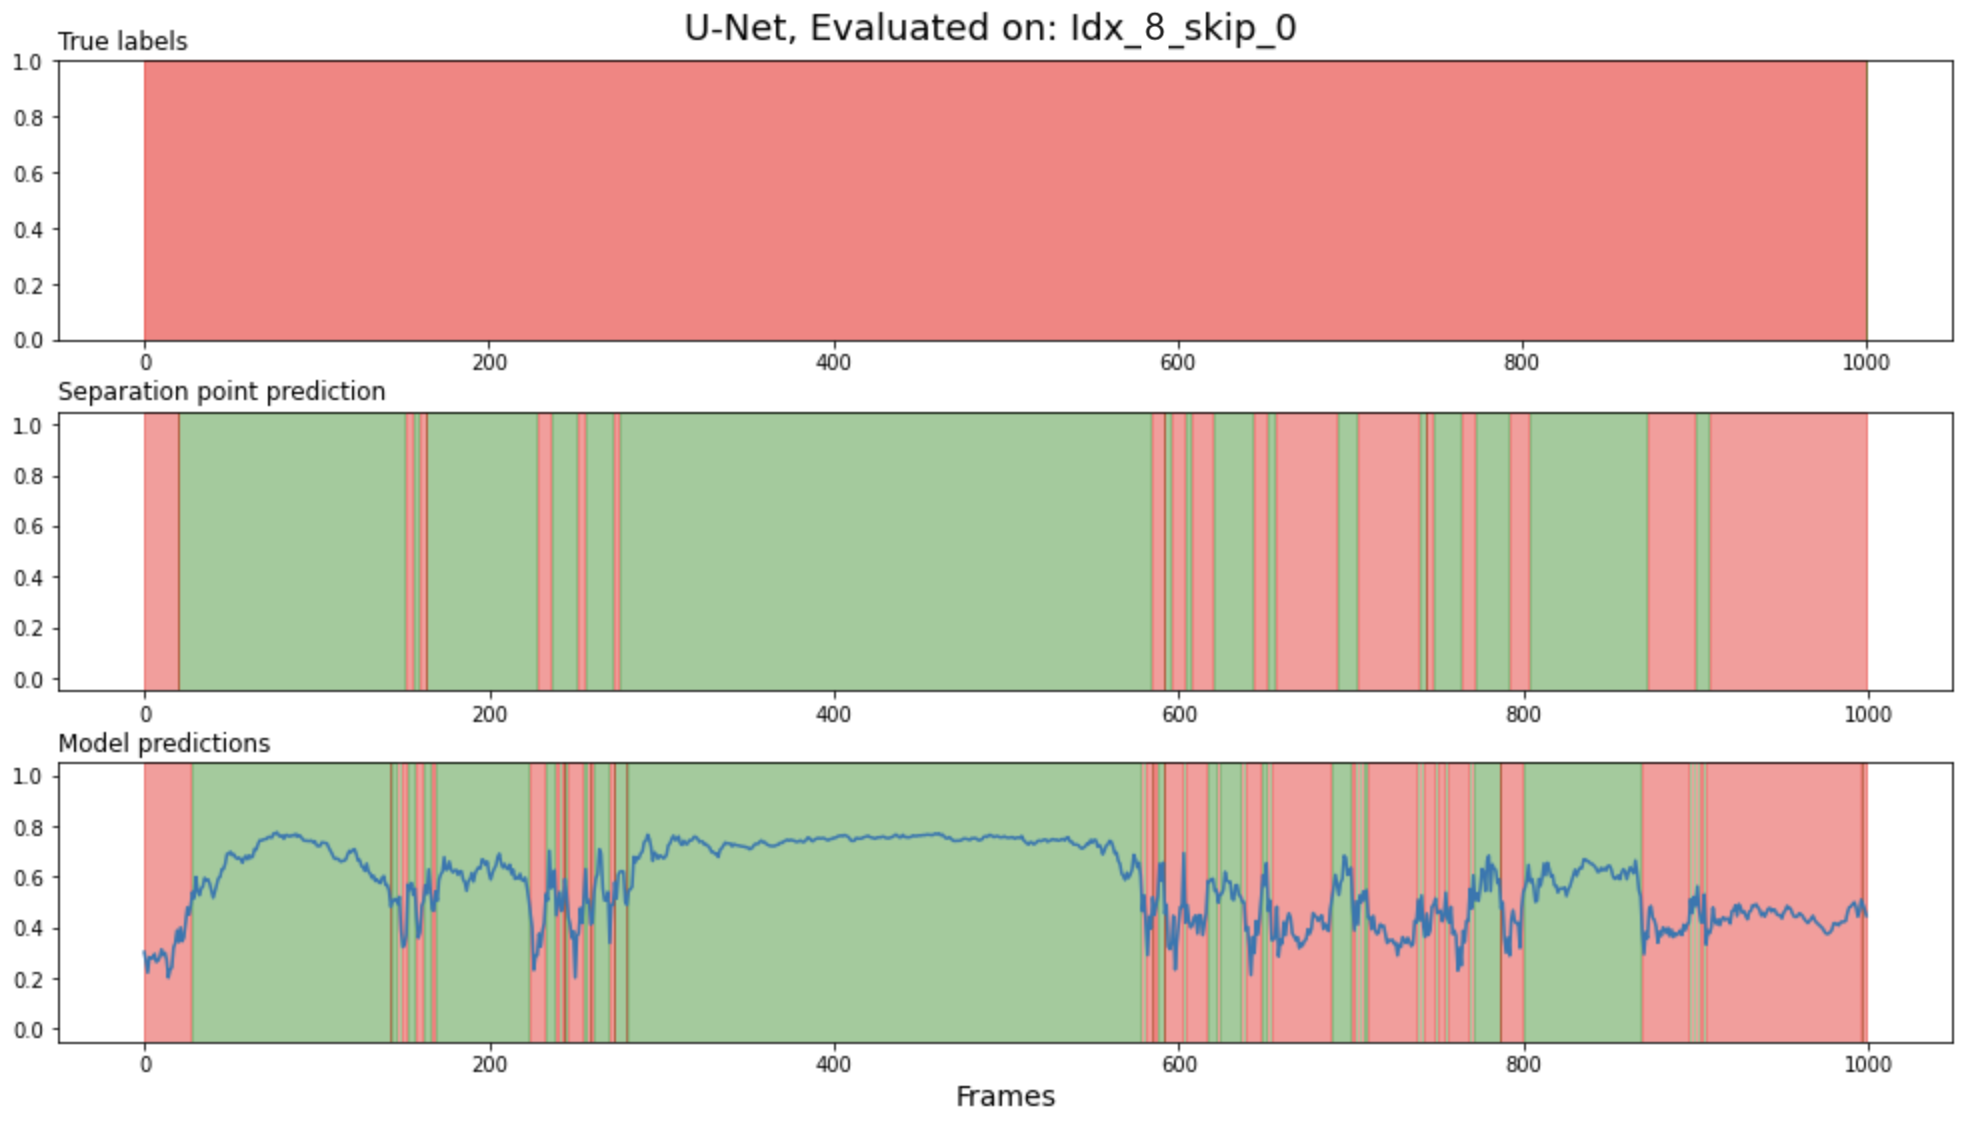
\includegraphics[width=\linewidth]{Materials/Results/UNet/unet4}
	\end{subfigure}
	\caption{Results of 1D U-Net model.}
	\label{unetres2}
\end{figure}

This tendency of making inflamed frames healthy seem to continue as we see in \autoref{unetres2}. For the first prediction we see the U-Net model likes to add healthy predictions even if they are wrong. In the second prediction we see the U-Net model is quite reluctant to add inflammation predictions when the ResNet model predicts too many healthy frames.

Even though we have only looked at four predictions this is the general tendency of the U-Net predictions. The model adds healthy predictions to the ResNet predictions, and it is very reluctant to add inflammation predictions, while being very steady and not overly confident in its predictions. As the ResNet was overly predicting inflammation, the U-Net seems to have caught on to a correct tendency of missing healthy frames. Although it has not quite managed to make its predictions two continuous blocks, its predictions are not heavily oscillating, and thus seem to have have caught on to the continuity a little.
\subsection{U-Net predictions for treatment prediction}
With the new segmentations produced by the U-Net model, treatment prediction was attempted again. This time the same 1D ResNet model was used, but training consisted of 70 epochs with a learning rate of $10^{-4}$ and with $0.01$ weight decay. Cross entropy was used as loss function and Adam was used for optimization.

\begin{table}[H]
	\hspace{-2.7cm}
	\begin{tabular}{|c|c|c|c|c|c|c|c|c|c|c|c|c|c|c|c|c|c|c|c|c|c|c|c|c|c|}
		\hline
		Idx&1
		&7
		&8
		&14
		&15
		&16
		&17
		&18
		&19
		&20
		&21
		&22
		&23
		&24
		&25
		&26
		&27
		&28
		&29
		&30
		&31
		&32
		&33
		&34
		&35\\\hline\hline
		Predictions&0
		&2
		&1
		&2
		&2
		&2
		&1
		&1
		&1
		&1
		&1
		&2
		&1
		&1
		&1
		&0
		&1
		&1
		&1
		&0
		&2
		&0
		&2
		&2
		&2\\\hline
		True&1
		&3
		&3
		&4
		&2
		&2
		&2
		&1
		&1
		&2
		&2
		&2
		&2
		&1
		&0
		&0
		&0
		&1
		&0
		&0
		&0
		&0
		&2
		&2
		&2\\\hline
	\end{tabular}
	\caption{Training a model only on the predicted U-Net segmentations, we find the following treatment predictions and true treatments shown for each video. The treatment classes are: 0 being 'healthy', 1 being 'local 5-ASA', 2 being 'Oral steroid', 3 being 'IV steroid' and 4 being 'oral 5-ASA'.}
	\label{unetPredsTreatmentTable}
\end{table}

\begin{figure}[H]
	\centering
	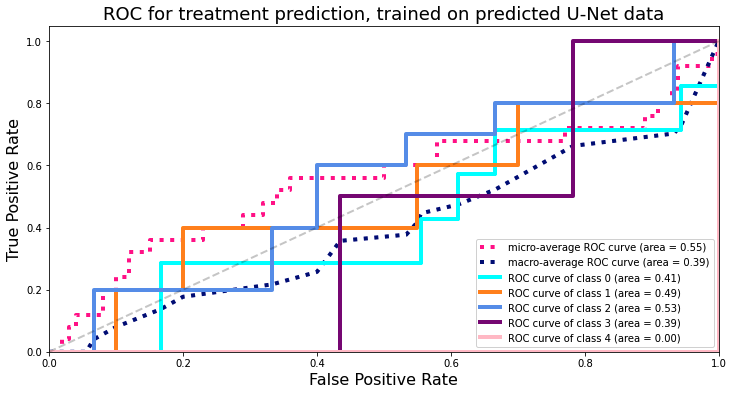
\includegraphics[width=0.85\linewidth]{Materials/Results/UNet/UNetROC1}
	\caption{ROC curves and area under the curve for the five binary 'one-vs-rest' classifiers along with micro- and macro-averages. Training was performed only on predicted segmentations.}
	\label{rocunetpreds}
\end{figure}
In \autoref{unetPredsTreatmentTable} we see the predicted treatments along the true prescribed treatment when we train only on the predicted segmentations from the U-Net model. In contrast to the previous results we now see predictions of classes $0, 1$ and $2$, where we previously did not see any predictions of treatment $1$. We also see an improvement in accuracy as we now have $52\%$.\\
Five binary 'one-vs-rest' classifiers were also trained for these predictions, and they were again trained using the same parameters as the multi class classifier. In \autoref{rocunetpreds} we see ROC curves for these binary classifiers, and we note the area under the curves being either $0.5$ or $0.4$ for all classes except class 4 which has $0.0$, which is significantly worse than for the previous treatment predictions.

When we include the true segmentations to the training data and repeat the experiment with the same parameters, we find the results seen in \autoref{unetPredsTrueTreatmentTable}. Here we again see the model predicting three classes, however, the accuracy drastically drops to $20\%$.

\begin{table}[H]
	\hspace{-2.7cm}
	\begin{tabular}{|c|c|c|c|c|c|c|c|c|c|c|c|c|c|c|c|c|c|c|c|c|c|c|c|c|c|}
		\hline
		Idx&1
		&7
		&8
		&14
		&15
		&16
		&17
		&18
		&19
		&20
		&21
		&22
		&23
		&24
		&25
		&26
		&27
		&28
		&29
		&30
		&31
		&32
		&33
		&34
		&35\\\hline\hline
		Predictions&2
		&2
		&2
		&2
		&1
		&1
		&1
		&2
		&2
		&2
		&1
		&1
		&2
		&2
		&1
		&2
		&2
		&2
		&2
		&2
		&1
		&0
		&2
		&1
		&2\\\hline
		True&1
		&3
		&3
		&4
		&2
		&2
		&2
		&1
		&1
		&2
		&2
		&2
		&2
		&1
		&0
		&0
		&0
		&1
		&0
		&0
		&0
		&0
		&2
		&2
		&2\\\hline
	\end{tabular}
	\caption{Training a model on the predicted U-Net segmentations and the true segmentations, we find the following treatment predictions and true treatments shown for each video. The treatment classes are: 0 being 'healthy', 1 being 'local 5-ASA', 2 being 'Oral steroid', 3 being 'IV steroid' and 4 being 'oral 5-ASA'.}
	\label{unetPredsTrueTreatmentTable}
\end{table}

In \autoref{rocunetpredstrue} we see the ROC curves when we add the true segmentations. Here, however, we see the area under the curve for class $0$ being a fair bit above $0.5$, indicating predictions for class $0$ are not random, while classes $1$ and $2$ are slightly above $0.5$. 

\begin{figure}[H]
	\centering
	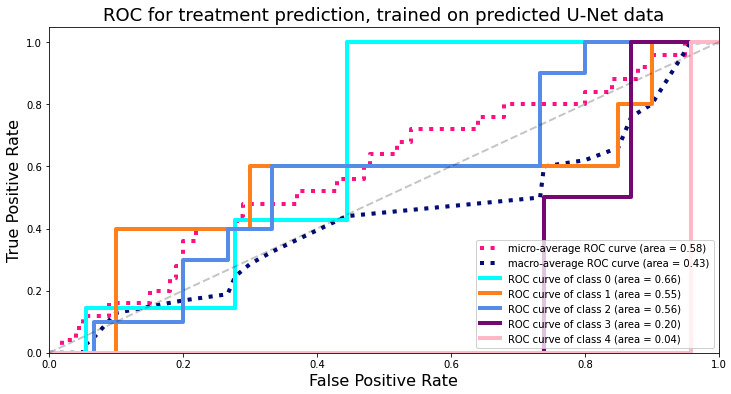
\includegraphics[width=0.85\linewidth]{Materials/Results/UNet/UNetROC2}
	\caption{ROC curves and area under the curve for the five binary 'one-vs-rest' classifiers along with micro- and macro-averages. Training was performed only on predicted segmentations.}
	\label{rocunetpredstrue}
\end{figure}